%-----------------------------
% B A C H E L O R A R B E I T
%-----------------------------



% DOKUMENTEINSTELLUNGEN
% ---------------------

% Dokumentenklasse
	\documentclass[11pt,twoside]{scrbook}
	%\usepackage{scrhack}
% Seitengeometrie
	\usepackage[a4paper,
				top=2.5cm,
				bottom=3.25cm,
				inner=3.75cm,
				outer=2.5cm
			   ]{geometry}
% Enkodierung
	\usepackage[utf8]{inputenc} %Linux
	%\usepackage[latin1]{inputenc} %Windows
	\usepackage[T1]{fontenc}
% Schriftart
	\usepackage{lmodern}
	\usepackage{dsfont}
% verwendete Sprachen
	\usepackage[english]{babel}



% ZUSÄTZLICHE PAKETE LADEN
% ------------------------

% BibTeX Quellenangaben
	\usepackage[numbers]{natbib}
% Mathematik Pakete
	\usepackage{amsmath}
	\usepackage{amsfonts}
	\usepackage{amssymb}
	\usepackage{fixmath}
	%\usepackage{amsthm}
% Grafiken/Floats einbinden
	\usepackage{graphicx}
	\usepackage[labelformat=empty]{subfig}
	\usepackage{wrapfig}
	%\usepackage{float}
% angepasste enumerate-Umgebungen

% Zeilenabstände anpassen
	%\usepackage{setspace}
% Seiten im Querformat
	%\usepackage{lscape}
% Seiten aus anderen PDFs einbinden
	%\usepackage[final]{pdfpages}
% Absolute Positionierung von Objekten auf Seiten
	\usepackage[absolute]{textpos}
% Informatik Pakete
	\usepackage{listings}
	\lstloadlanguages{C++}
	\usepackage{color}
	%\usepackage{url}
% Schönere Seitenheader
	\usepackage{fancyhdr}
% Leerzeichen am Ende von Abkürzungen
	\usepackage{xspace}
% für \C++ benötigt
	\usepackage{relsize}
% Initiale
	%\usepackage{lettrine}
% benötigt für kontinuierliche Fußnotennummerierung
	\usepackage{chngcntr}
% Zeilenumbrüche in Wortzusammensetzungen, die - enhalten
	\usepackage{hyphenat}
% Aufzählung	
	\usepackage{paralist}
	
% neuster SHIT
	\usepackage{bbm}
	\usepackage{booktabs}
	\usepackage{float}
	\usepackage{rotating}
	\usepackage{mdframed}
	\usepackage{morefloats}


% pdfLaTeX ERWEITERUNGEN
% ----------------------

% Mikrotypographie Features benutzen
	\usepackage{microtype}
% Links aus der Inhaltsverzeichnis etc.
	\usepackage[pdfborder={0 0 0},
				pdftitle={Bachelorarbeit},
				pdfsubject={Monte Carlo Methoden in der statistischen Physik und ihre Anwendung zur Simulation von Spinsystemen},
				pdfauthor={Robert Rüger}
			   ]{hyperref}
% Links auf den Beginn von Floats statt auf die Beschriftung
	\usepackage[all]{hypcap}



% BENUTZERDEFINIERTES AUSSEHEN
% ----------------------------

% Verbot von Hurenkindern und Schusterjungen?
	%\clubpenalty = 10000
	%\widowpenalty = 10000
	%\displaywidowpenalty = 10000
% FancyHDR Stil
	\pagestyle{fancy}
	\fancyhf{}
	\fancyfoot[EL,OR]{\small \thepage}
	\fancyhead[EL]{\footnotesize \leftmark}
	\fancyhead[OL]{\footnotesize \rightmark}
	\renewcommand{\headrulewidth}{0.4pt}
	\renewcommand{\footrulewidth}{0.4pt}
% Obere Seitenbeschriftungen
	\renewcommand{\chaptermark}[1]{\markboth{Kapitel \thechapter\hskip 12pt #1}{}}
	\renewcommand{\sectionmark}[1]{\markright{\thesection\hskip 8pt #1}}
% GROSSBUCHSTABEN in den Headern (fieser Hack wegen gleichzeitiger Verwendung vom babel Paket ...)
	\let\markrightOld\markright
	\renewcommand{\markright}[1]{\markrightOld{\MakeUppercase{#1}}}
	\let\markbothOld\markboth
	\renewcommand{\markboth}[1]{\markbothOld{\MakeUppercase{#1}}}
% Seitenumbrüche in Formeln
	%\allowdisplaybreaks[1]
% kein Rand in fboxes
	\setlength{\fboxsep}{0pt}
% Zeilen und Absatzabstand
	%\onehalfspacing
	\linespread{1.1}
	% einfacher Zeilenabstand in Fußnoten
	\let\footnoteOld\footnote
	\renewcommand{\footnote}[1]{\linespread{0.95}\footnoteOld{#1}}
	%\setlength{\parskip}{5pt}
% kontinuierliche Fußnotennummerierung (nicht in jedem Kapitel von vorn beginnen ...)
	\counterwithout{footnote}{chapter}
% DIN 1505 Literaturverzeichnis
	\bibliographystyle{alphadin}
	%\bibliographystyle{halpha}
% Mehr Platz in Tabellen (beeinflusst auch Matrizen!)
	%\setlength{\tabcolsep}{3pt}
	%\renewcommand{\arraystretch}{1.2}
% Fett gedruckte Nummern bei Aufzählungen
	\renewcommand{\labelenumi}{\textbf{\theenumi.}}
% Überall Schrift mit Serifen benutzen
	\renewcommand{\sfdefault}{\rmdefault}
% Quellcode
\definecolor{listinggray}{gray}{0.9}
\definecolor{lbcolor}{rgb}{0.9,0.9,0.9}
\lstset{
backgroundcolor=\color{lbcolor},
    tabsize=4,    
%   rulecolor=,
    language=[GNU]C++,
        basicstyle=\scriptsize,
        upquote=true,
        aboveskip={1.5\baselineskip},
        columns=fixed,
        showstringspaces=false,
        extendedchars=false,
        breaklines=true,
        prebreak = \raisebox{0ex}[0ex][0ex]{\ensuremath{\hookleftarrow}},
        frame=single,
        numbers=left,
        showtabs=false,
        showspaces=false,
        showstringspaces=false,
        identifierstyle=\ttfamily,
        keywordstyle=\color[rgb]{0,0,1},
        commentstyle=\color[rgb]{0.026,0.112,0.095},
        stringstyle=\color[rgb]{0.627,0.126,0.941},
        numberstyle=\color[rgb]{0.205, 0.142, 0.73},
%        \lstdefinestyle{C++}{language=C++,style=numbers}’.
}
\lstset{
    backgroundcolor=\color{lbcolor},
    tabsize=4,
  language=C++,
  captionpos=b,
  tabsize=3,
  frame=lines,
  numbers=left,
  numberstyle=\tiny,
  numbersep=5pt,
  breaklines=true,
  showstringspaces=false,
  basicstyle=\footnotesize,
%  identifierstyle=\color{magenta},
  keywordstyle=\color[rgb]{0,0,1},
  commentstyle=\color{Darkgreen},
  stringstyle=\color{red}
  }
		



% BENUTZERDEFINIERTE BEFEHLE
% --------------------------


% Horizontale Linie
	\newcommand{\HRule}{\rule{0.97\linewidth}{0.4mm}}


% Grad Symbol
	\newcommand{\degree}{\ensuremath{^\circ}}

	
I
% Hilbertraumvektoren
	\newcommand{\ket}[1]{\left| #1 \right>}
	\newcommand{\bra}[1]{\left< #1 \right|}
	\newcommand{\braket}[2]{\left< #1 \vphantom{#2} \right| \left. \hskip -3pt #2 \vphantom{#1} \right>}
	\newcommand{\matrixel}[3]{\left< #1 \vphantom{#2#3} \right| #2 \left| #3 \vphantom{#1#2} \right>}
% Vektoren Dick Notation
	\renewcommand{\vec}[1]{\mathbf{#1}}



% BEGINN DES DOKUMENTS
% --------------------
	\begin{document}



% Titelseite
% ----------
	\begin{titlepage}
%\enlargethispage{0.4cm}
\HRule \vskip 4.5cm

\begin{textblock}{5}(10.25,1.85)
	\includegraphics[width=4.5cm]{./figures/uni-logo.pdf}
\end{textblock}

\begin{center}

\begin{LARGE}
	\textsc{Bachelor Thesis}
\end{LARGE}\vskip 1.5cm

\begin{huge}
\textbf{Band structure studies of graphene and modified graphene structures }
\end{huge}\vskip 2cm

\begin{LARGE}
	\textbf{Dirk Hornung}
\end{LARGE}\vskip 2.75cm

\begin{LARGE}
	Institut für Theoretische Physik\\
	Johann Wolfgang Goethe-Universität\\
	Frankfurt am Main \vskip 0.66cm
	September 2014
\end{LARGE}

\end{center}
\vfill

\begin{minipage}{5.5cm}
	\begin{flushright}
		\begin{large}
			First proofreader:\\
			
		\end{large}
	\end{flushright}
\end{minipage}\hskip 0.5cm
\begin{minipage}{6cm}
	\begin{flushleft}
		\begin{large}
			Prof.~Dr.~Roser Valent\'{\i}\\
			
		\end{large}
	\end{flushleft}
\end{minipage}\vskip 0.4cm

\begin{minipage}{5.5cm}
	\begin{flushright}
		\begin{large}
			Second proofreader:\\
			
		\end{large}
	\end{flushright}
\end{minipage}\hskip 0.5cm
\begin{minipage}{6cm}
	\begin{flushleft}
		\begin{large}
			Prof.~Dr.~Eberhard Engel\\
			
		\end{large}
	\end{flushleft}
\end{minipage}\vskip 0.4cm

\HRule
\end{titlepage}



% Inhaltsverzeichnis
% ------------------
	\setcounter{secnumdepth}{3}
	\setcounter{tocdepth}{3}
	\addtocontents{toc}{\protect\thispagestyle{empty}}
	\pagestyle{empty}
	\tableofcontents
	\cleardoublepage
	\pagestyle{fancy}
	

% Kapitel
% -------
	\chapter{Introduction}
	The experimental and theoretical study of graphene is a very rapid growing field in modern physics (\ref{fig:grapheneManuscripts}), which is mainly because of the physical milestones of Andre Geim and Konstantin Novoselov. They discovered the first true 2D crystal ever observed in nature : \textbf{graphene}. Both got credited from the Royal Swedish Academy of Science with the Nobel Prize in Physics (2010). The existence of graphene-like materials has often been doubted due to the \textit{Mermin-Wagner theroem}, which states that a 2D crystal melts at any small but non zero temperature. Graphene has the thickness of only one atom and is nevertheless stable, though many believed it was impossible for such a thin crystalline material to be stable. Furthermore graphene, which is based on carbon has some very powerful properties. It is the thinnest, but also strongest known material with the best heat conductivity. It is transparent, conducts electricity as good as copper and is yet so dense, that not even Helium can pass it. The electrons in graphene show relativistic behavior and thus it can be an ideal candidate for proving theoretical quantum-field models. Moreover graphene can be used as transistors faster by far than common silicon ones. In addition its properties of transparency and conductivity combined with the enormous stability and thickness make it a perfect material for new touch screens, light panels or even solar cells. \\
	\begin{figure}[H]
		\centering
		\includegraphics[width=0.7\textwidth]{figures/Introduction/grapheneManuscripts.png}
		\caption{Number of manuscripts with the title 'graphene' posted on www.arxiv.org from the years 2005 to 2013. As one can see, there is an exponential growth from 2005-2008 and a climax right after awarding the nobel prize in 2010.}
		\label{fig:grapheneManuscripts}
	\end{figure}
	\begin{figure}[h]
		\centering
		\includegraphics[width=0.7\textwidth]{figures/Introduction/Graphen.jpg}
		\caption{Graphene lattice. Figure taken from \cite{deWikiGraphen}. }
	\end{figure}	
	\noindent As the manufacturing of graphene is a complicated process one can never exclude impurities. In the following chapters we will discuss the effect of some basic impurities in a graphene lattice. We will start with an introduction to solid state physics and continue with some details about carbon materials. Later on we will discuss the calculations made from the density functional theory and the tight binding model.
	\chapter{Fundamental concepts in a solid state}
	In this section we follow \cite{Festkoerperphysik_Ashcroft} and \cite{Festkoerperphysik_RG_AM}.\\\\
	For describing a crystal and its properties some solid state physic theory is needed. We therefore want to introduce some fundamental basics, starting with lattice descriptions and ending with a better understanding of band structures and density of states.
	\section{Crystal lattice}
		Solid state physics basically addresses the description of crystal properties. A crystal is described in forms of a Bravais lattice (discussed below) and of an atomic basis attached at each lattice point.
			
		\subsection{Bravais lattice}
			A \textit{Bravais} lattice defines the periodic basis of a crystal as a lattice. This basis can consist of atoms, ions, molecules et cetera. The d dimensional \textit{Bravais} lattice is given by 
			\begin{align}
				\label{eq:bravais}
				\vec{R} = \sum_{i=1}^{d} n_i \vec{a_i} && n_i \in \mathbb{Z},
			\end{align}
			where $\vec{a_i}$ are arbitrary vectors with the condition that $\vec{a_i}$ and $\vec{a_j}$ ($i \neq j$) are linearly independent. With equation (\ref{eq:bravais}) we now can reach every unit in a solid by adjusting $n_i$. In most cases we will have a 3-dimensional lattice, i.e. with $d=3$.
			
		
		\subsection{Primitive Cell}
			\label{sec:primitiveCell}
			Due to the periodicity of the crystal we can focus on the primitive cell, defined a volume in the position space that contains exactly one lattice point and fills the whole space when translated among the \textit{Bravais} vectors $a_i$. 
			It is not unique, i.e. it can have different shapes. Besides the primitive cell one can also build a conventional cell, that can contain more than one lattice point and which is the smallest form of a \textit{unit cell} (volume formed by the arbitrary chosen basis vectors). 
	
		\subsection{Wigner-Seitz cell}
			It is always possible to choose a primitive cell with full symmetry of the \textit{Bravais lattice}. The most common method of choosing such a cell is the \textit{Wigner-Seitz} construction. To construct the two dimensional \textit{Wigner-Seitz cell} one picks a lattice point and draws lines to all neighbor lattice points. For each line the perpendicular bisecting plane has to be constructed and the encased plane is the \textit{Wigner-Seitz cell}. The two dimensional construction is analogous to the three dimensional case.			
			
		\subsection{Reciprocal lattice}
			\label{sec:reciprocalLattice}
			Making use of periodicity one can also change into the \textit{reciprocal lattice}. Consider a plane wave $e^{i\vec{k \cdot r}}$ and the set of vectors $\vec{R}$, which form a \textit{Bravais lattice}. The set of all wave vectors $\vec{k}$, that generate plane waves with the periodicity of the \textit{Bravais lattice}, are called \textit{reciprocal lattice}.
			\begin{equation}
				\label{eq:reciprocalLattice}
				e^{i\vec{k}(\vec{r + R})} = e^{i \vec{k \cdot r}}
			\end{equation}
			By dividing through $e^{i\vec{k \cdot r}}$ we obtain the following condition
			\begin{equation}
				e^{i\vec{k \cdot R}} = 1.
			\end{equation}
			Moreover the reciprocal lattice is a Bravais lattice spanned by
			\begin{equation}
				\vec{k_i} = 2 \pi \epsilon_{ijk} \frac{\vec{a_j \times a_k}}{|\vec{a_1 \cdot (a_2 \times a_3})|},
			\end{equation}
			where we used the \textit{Einstein notation} and the \textit{Levi-Cevita symbols}. \\
			The above equation can also be transformed to the following condition :
			\begin{equation}
				\label{eq:reciprocalCondition}
				\vec{a_i} \cdot \vec{b_j} = 2 \pi \delta_{ij}.
			\end{equation}
			The reciprocal lattice can now be written as 
			\begin{align}
				\label{eq:reciprocalLattice2}
				\vec{k} = h\vec{b_1} + k\vec{b_2} + l\vec{b_3} && h,k,l \in \mathbb{Z},
			\end{align}	
			We will see that the integers h,k and l denote the \textit{Miller indices}. In addition, there exists a \textit{Wigner-Seitz cell} for the \textit{reciprocal lattice} called \textit{Brillouin zone}. 	
			
		\subsection{Brillouin zone}
			For band structure calculations it is essential to use the \textit{Brillouin zone}. For periodical crystals the energy structure is periodic within every \textit{Brillouin zone}. Thus we only have to calculate properties in one \textit{Brillouin zone} and can transfer the result to the whole lattice.
	
	\section{Many body Hamiltonian}
		To deal with modern many-body problems we have to use quantum mechanics, starting with the \textit{Schrödinger equation} for a certain Hamiltonian ,whose general form is given by the total kinetic energy and potential.
		\begin{equation}
			\label{eq:generalHamiltonian}
			\hat H = \hat T + \hat V.
		\end{equation}
		In solids we only have to regard Coulomb repulsion between nuclei and electrons. As a consequence we have to handle three different types of interaction :\\
		\begin{compactenum}[I]
			\item Nucleus-nucleus interaction
				\begin{equation}
					V_{nn} = \sum_{I \neq J}^{N_n} \frac{e^2}{8 \pi \epsilon_0} \frac{Z_I \cdot Z_J}{|\vec{R_I - R_J}|},
				\end{equation}
				
				
			\item Nucleus-electron interaction
				\begin{equation}
					V_{ne} = \sum_{I}^{N_n} \sum_{i}^{N_e} \frac{e^2}{4 \pi \epsilon_0} \frac{Z_I}{|\vec{R_I - r_i}|},
				\end{equation}
				
			\item Electron-electron interaction
				\begin{equation}
					V_{ee} = \sum_{i \neq i}^{N_e} \frac{e^2}{8 \pi \epsilon_0} \frac{1}{|\vec{r_i - r_j}|}.
				\end{equation}
		\end{compactenum}
		By adding the total kinetic energy we obtain the searched Hamiltonian of a many body solid.
		\begin{equation}
			\label{eq:manyBodyHamiltionian}
			\begin{split}
				\hat H &= \hat T_n + \hat T_e + \hat V_{nn} + \hat V_{ne} + \hat V_{ee} \\
				&= \sum_{I}^{N_n}\frac{h^2}{2m_I} \nabla_I^2 + \frac{h^2}{2m_e} \sum_{i}^{N_e} \nabla_i^2 + \frac{e^2}{4 \pi \epsilon_0} \left[ \sum_{I \neq J}^{N_n} \frac{1}{2} \frac{Z_I \cdot Z_J}{|\vec{R_I - R_J}|} + \sum_{I}^{N_n} \sum_{i}^{N_e}  \frac{Z_I}{|\vec{R_I - r_i}|} + \sum_{i \neq i}^{N_e} \frac{1}{2} \frac{1}{|\vec{r_i - r_j}|} \right]
			\end{split}	
		\end{equation}
		 The solution of Equation (\ref{eq:manyBodyHamiltionian}) poses serious difficulty. As a result we need to introduce several approximations like the \textit{Born-Oppenheimer approximation} to get a solvable formalism. But first we want to introduce the \textit{atomic units}, that will shorten the following equations by loosing cumbersome combinations of the fundamental constants h, m, e and $\epsilon_0$.

	\section{Atomic units}
		\label{sec:atomicUnits}
		As we are dealing with very small scales the SI units of energy (J) and length (m) are inappropriate. A more natural unit system to employ for this problem is the \textit{atomic units}.
		In \textit{atomic units} the energy and the lenght are measured in terms of Hartree energy and the Bohr radius.
		\begin{gather}
			a_0 = \frac{4 \pi \epsilon_0 \hbar^2}{m_e e^2} \\
			E_h = \frac{\hbar^2}{m_e a_0^2} = \frac{e^2}{4 \pi \epsilon_0}		
		\end{gather}
		In addition one can write :
		\begin{equation}
			\label{eq:atomicUnits}
			e = m_e = \hbar = \frac{1}{4\pi\epsilon_0} = 1.
		\end{equation}
		If we apply Equation \ref{eq:atomicUnits} to our many body Hamiltonian we get 
		\begin{equation}
				\hat H = \sum_{I}^{N_n}\frac{1}{2} \nabla_I^2 + \frac{1}{2} \sum_{i}^{N_e} \nabla_i^2 + \sum_{I \neq J}^{N_n} \frac{1}{2} \frac{Z_I \cdot Z_J}{|\vec{R_I - R_J}|} + \sum_{I}^{N_n} \sum_{i}^{N_e}  \frac{Z_I}{|\vec{R_I - r_i}|} + \sum_{i \neq i}^{N_e} \frac{1}{2} \frac{1}{|\vec{r_i - r_j}|}.
		\end{equation}	

	\section{Born-Oppenheimer approximation}
		\label{sec:bornOppenheimer}
		Due to the large difference between the electron and the nuclei mass, one can assume the atomic cores have a fixed position and neglect their kinetic energy, leading to an easier to handle Hamiltonian.
		\begin{equation}
			\hat H = \hat T_e + \hat V_{nn} + \hat V_{en} + \hat V_{ee}		
		\end{equation}
		$V_{nn}$ and $V_{en}$ are taken together to a new variable called external potential $V_{ext}$.
		\begin{equation}
			\begin{split}
				\hat H &= \hat T_e + \hat V_{ee} + \hat V_{ext} \\
				\hat H &= \frac{1}{2} \sum_{i}^{N_e} \nabla_i^2 + \sum_{i \neq i}^{N_e} \frac{1}{2} \frac{1}{|\vec{r_i - r_j}|} + \sum_{I}^{N_n} \sum_{i}^{N_e}  \frac{Z_I}{|\vec{R_I - r_i}|}  			
			\end{split}
		\end{equation}
				
	\section{Electronic band theory}
		With the use of a periodical lattice we can summarize the electron-electron correlation $V_{ee}$ and the external potential $V_{ext}$ given by the fixed lattice ions into an effective potential 
		\begin{equation}
			V_{eff}(\vec r) = \sum_i v(\vec r_i).
		\end{equation}		
		\subsection{Bloch theorem}
			\label{sec:bloch}
			We now want to describe electrons in a periodical potential. Instead of using plane waves for the eigenstates of the Hamiltonian (as used for a free electron gas, without a positive ion structure) we have to use lattice specific modulated plane waves.	For a Bravais lattice with a periodical potential one can rewrite the eigenstates $\psi$ of the one-electron Hamiltonian
			\begin{align}
				\hat H = -\frac{ \hbar^2 \nabla^2}{2m_e} + V(\vec{r}) && \text{ with } V(\vec{r + R}) = V(\vec{r})
			\end{align}
			as a product of a plane wave and a periodic function $u_k(\vec{r})$.
			\begin{align}
				\label{eq:bloch}
				\psi(\vec{r}) = e^{i\vec{k \cdot r}} u_k(\vec{r}) && \text{ with } u_k(\vec{r + R}) = u_k(\vec{r})
			\end{align}	
		Evolving the wave function into orthonormal orbitals
		\begin{equation}
			| \phi \rangle = \sum_{\alpha} C_\alpha |\psi_\alpha \rangle 
		\end{equation}
		and making use of the \textit{Schrödinger equation} we obtain: 
		\begin{equation}
			\begin{split}
				\label{eq:blochSchroedinger}
				\hat H | \psi_\alpha \rangle &= \epsilon_\alpha | \psi_\alpha \rangle \\
				( \hat T + \hat V_{eff}) | \psi_\alpha \rangle &= \epsilon_\alpha | \psi_\alpha \rangle \\
				\langle k | (\hat T + \hat V_{eff}) | \psi_\alpha \rangle &= \epsilon_\alpha \langle k | \psi_\alpha \rangle \\
				\langle k | (\hat T + \hat V_{eff}) | \psi_\alpha \rangle &= \epsilon_\alpha C_\alpha(k) \\
				\langle k | \hat T | \psi_\alpha \rangle + \langle k | \hat V_{eff} | \psi_\alpha \rangle &= \epsilon_\alpha C_\alpha(k),
			\end{split}
		\end{equation}
		With the help of the completeness relation we will find solutions for $\langle k | \hat T | \psi \rangle$ and $ \langle k | \hat V_{eff} | \psi \rangle $. 
		\begin{equation}
			\begin{split}
				\langle k | \hat T | \psi_\alpha \rangle &= \epsilon_{kin} \langle k | \psi_\alpha \rangle \\
				&= \frac{\hbar^2 k^2}{2 m} C_\alpha(k)
			\end{split}
		\end{equation}
		\begin{equation}
			\begin{split}
				\langle k | \hat V_{eff} | \psi \rangle &= \int_{-\infty}^{\infty} dk' \langle k | \hat V_{eff} | k' \rangle \langle k' | \psi_\alpha \rangle \\
				&= \int_{-\infty}^{\infty} \langle k | \hat V_{eff} | k' \rangle C_\alpha(k')
			\end{split}
		\end{equation}
		Before evaluating $\langle k | \hat V_{eff} | \psi_\alpha \rangle$ we have to regard $\langle k | \hat V_{eff} | k' \rangle$.
		\begin{equation}
			\begin{split}
				\label{eq:kVk'}
				\langle k | \hat V_{eff} | k' \rangle &= \int_{-\infty}^{\infty} dx \int_{-\infty}^{\infty} dx' \langle k | x \rangle \langle x | \hat V_{eff} | x' \rangle \langle x' | k' \rangle \\
				&= \frac{1}{2\pi} \int_{-\infty}^{\infty} dx \int_{-\infty}^{\infty} dx' V_{eff}(x')\delta(x'-x) e^{i(k'x'-kx)} \\
				&= \frac{1}{2\pi}\int_{-\infty}^{\infty} dx V_{eff}(x) e^{ix(k'-k)}
			\end{split}
		\end{equation}
		In the last line we used the spatial illustration of the impulse eigenfunctions 
		\begin{equation}
			\begin{split}
				\label{eq:impulsTransformation}
				\langle x | k \rangle = \frac{1}{\sqrt{2 \pi}} e^{ikx} \\
				\langle k | x \rangle = \frac{1}{\sqrt{2 \pi}} e^{-ikx},
			\end{split}
		\end{equation}	
		and the orthogonality of $\langle x | x' \rangle$.
		\begin{equation}
			\langle x | \hat V_{eff} | x' \rangle = V_{eff}(x) \langle x | x' \rangle = V_{eff}(x) \delta(x-x')
		\end{equation}
		To solve the integral in Eq. \ref{eq:kVk'} we furthermore need to use the Fourier transformation 
		\begin{gather}
			\mathcal{F}[f(t)] = \int_{-\infty}^{\infty} f(t) e^{-i\omega t} dt \\
			f(t) = \mathcal{F}^{-1} = \frac{1}{2 \pi} \int_{-\infty}^\infty \mathcal{F}(\omega) e^{i\omega t} d\omega,
		\end{gather} 
		which will lead us to :
		\begin{equation}
			\begin{split}
				\langle k | \hat V | k' \rangle &= \sum_{n=-\infty}^{\infty} \int_{-\infty}^{\infty} dx V_n e^{ix(k' - k - k_n)} \\
				&= \sum_{n=0}^{\infty} V_n \delta(k' - k - k_n).
			\end{split}
		\end{equation}
		Applying the last equation to $\langle k | \hat V_{eff} | \psi_\alpha \rangle$ will give us the last missing part of the \textit{Schrödinger equation}. 
		\begin{equation}
			\langle k | \hat V_{eff} | \psi_\alpha \rangle = \sum_{n=-\infty}^{\infty} V_n  C_\alpha(k + k_n)
		\end{equation}
		Putting all together into Eq. \ref{eq:blochSchroedinger} we have
		\begin{equation}
			\begin{split}
				\frac{\hbar^2 k^2}{2m} C_\alpha(k) + \sum_{n=-\infty}^{\infty}V_n C(k +k_n) &= \epsilon C_\alpha(k) \\
				\frac{\hbar^2 k_i^2}{2m} C_\alpha(k_i) + \sum_{n=-\infty}^{\infty}V_n C_\alpha(k_{i+n}) &= \epsilon C_\alpha(k_i).
			\end{split}
		\end{equation}
		This is an $\infty$-dimensional eigenvalue problem. 
		\begin{equation}
			\label{eq:blochEigenvalue}				
			\begin{pmatrix}
				\frac{\hbar^2 k_0^2}{2 m} + V_0 & V_1 & V_2 & \dots \\
				V_{-1} & \frac{\hbar^2 k_1^2}{2 m} + V_0 & V_1 & \dots \\
				V_{-2} & V_-1 & \frac{\hbar^2 k_2^2}{2 m} + V_0  & \dots \\
				\vdots & \vdots & \vdots & \ddots	 	
			\end{pmatrix}
			\begin{pmatrix}
				C_\alpha(k_0) \\
				C_\alpha(k_1) \\
				C_\alpha(k_2) \\
				\vdots
			\end{pmatrix}
			= \epsilon
			\begin{pmatrix}
				C_\alpha(k_0) \\
				C_\alpha(k_1) \\
				C_\alpha(k_2) \\
				\vdots
			\end{pmatrix}.
		\end{equation}
		Additionally we have to complement the matrix with negative indices $k_{-i}$. \\
		The eigenvalues $\epsilon_\alpha$ therefore should be denoted by two numbers : the wave number k' in the first \textit{Brillouin zone} and a natural number n, which contains the particular number of the eigenvector.
		\begin{align}
			\epsilon_\alpha & \text{ with } \alpha \leftrightarrow k, n
		\end{align}	
		Moreover the eigenvalues $\epsilon_\alpha$ create a \textit{band structure} with several properties.
		\begin{enumerate}
			\item The eigenvalues are \textbf{periodic functions of the quantum numbers k}. It is sufficient to describe the \textit{band structure} in the first \textit{Brillouin zone}.
			\item $\epsilon_\alpha$ is limited and for an index n we are stuck with a restricted \textbf{bandwidth} and call the $\epsilon_{n, k}$ for an index n \textbf{energy band}.
			\item  The forbidden areas between two bands are called \textbf{band gaps} and can be used for distinguishing metals, semiconductors and isolators.
		\end{enumerate}
		
	\section{Density of states}
		For describing the properties of a solid state, we are also interested in the amount of states per energy, the so called \textit{density of states}, which is defined by the number of states per energy interval 
		\begin{equation}
			D(\epsilon) = \frac{1}{V} \sum_{\alpha \sigma} \delta (\epsilon - \epsilon_\alpha) = \frac{1}{V} \sum_{k n \sigma} \delta (\epsilon - \epsilon_{k,n}), 
		\end{equation}
		where V is the total volume of the solid state, d is the dimension and $\sigma$ is needed for the electron spin consideration. If the k-point density is high enough we can turn the sum into an integral.
		\begin{equation}
			D(\epsilon) = \frac{1}{V} \sum_k \sum_{n \sigma} \delta (\epsilon - \epsilon_\alpha) \rightarrow \frac{1}{V^d} \frac{V^d}{(2\pi)^d} \sum_{n \sigma} \int d\vec k \delta (\epsilon - \epsilon_{k,n}) 
			\label{eq:dosInt}	
		\end{equation} 
		To simplify the integral we can rewrite the Dirac delta into a \textit{Heaveside function}.
		\begin{equation}
			\delta(\epsilon - \epsilon_{kn})d\epsilon = \Theta = ( \epsilon < \epsilon_{k,n} < \epsilon +d\epsilon)
		\end{equation}
		As a consequence one only receives a contribution when the energy is in between the energy interval $[\epsilon, \epsilon + d\epsilon$.
		\begin{equation}
			D(\epsilon) d\epsilon = \frac{1}{(2\pi)^d} \sum_{n \sigma} \int d\vec k \delta (\epsilon - \epsilon_{k,n})
		\end{equation} 
		Using $dk^d = dS dk_\perp$, with dS being the surface of a d-dimensional spheric in the reciprocal space and $dk_\perp$ being the corresponding normal vector, simplifies the above equation.
		\begin{equation}
			D(\epsilon) = \frac{1}{(2\pi)^2} \sum_{n \sigma} \int_{\partial S} \frac{d S}{|\nabla \epsilon_{k n}|} \Theta(\epsilon - \epsilon_{k n}),
		\end{equation}
		where $d\epsilon = |\nabla_{kn}| dk_\perp$.\\
		Having derived the needed basics we will continue with the \textit{density functional theory}.
		
		
			
		
		
	
		
	
	
		

	\chapter{Introduction to carbon materials}
	As graphene is composed of \textit{sp\textsubscript{2}-hybridized} carbon atoms we need want to introduce some fundamentals of the carbon properties.
	\section{Carbon Atom}
		Carbon is the $6^{th}$ element in the $14^{th}$ group of the periodic table (\ref{fig:periodicTable}). Therefore it is nonmetallic, tetravalent and constituted of 6 protons and electrons. There are three natural occurring isotopes, with $^{12}_{\phantom{0}6}C$, $^{13}_{\phantom{0}6}C$ being stable and $^{14}_{\phantom{0}6}C$ being radiative with an half life of 5.730 years. $^{14}_{\phantom{0}6}C$ $\beta$ decays to nitrogen and is used for historical dating. 
		The most common allotropes of Carbon are graphite, graphene and diamond. Diamond and graphene have the highest thermal conductivity of all known materials. The electron configuration in the ground state of carbon is $1s^22s^22p^2$, i.e. there are two electrons in the 1s orbital, which are irrelevant for chemical bondings, in addition to four electrons in the outer shell. The 2p orbital is roughly 4eV higher than the 2s orbital, therefore it is energetic favorable to put two electrons in the 2s and two electrons the 2p orbitals. However, carbon tends to fill one 2p orbital with an electron from the 2s orbital, in the presence of other atoms like H, O or C, which leads to 4 equal quantum states $|2s \rangle$, $|2p_x \rangle$, $|2p_y \rangle$ and $|2p_z \rangle$. A quantum-mechanical superposition of the state $|2s \rangle$ with $n |2p_i \rangle$ states is called sp\textsuperscript{n} hybridization.
		\begin{figure}[htbp]
			\begin{minipage}[b]{0.4\textwidth} 
				\includegraphics[width=\textwidth]{figures/Carbon/carbonAllotropes.png}		
			\end{minipage}
			% Auffüllen des Zwischenraums
			\hfill
			% minipage mit Grafik
			\begin{minipage}[t]{0.5\textwidth}
			\centering
			% \textwidth bezieht sich nun auf die Minipage
			\includegraphics[width=\textwidth]{figures/Carbon/carbonElectronicConfiguration.png}
			\end{minipage}
			\caption{\textbf{Left :} Allotropes of Carbon : a) diamond, b) graphite, c) Ionsdaleite, d-f) fullerences, g) amorphous carob, h) carbon, nanotube. Figure taken from \cite{enWikiAllotropesOfCarbon}. \\
			\textbf{Right :} Comparison between the electronic configuration of carbon in the ground state and in the excited state.}		
		\end{figure}

		\subsection{sp\textsuperscript{1}-hybridization}
			\begin{figure}[h]
				\centering
				\includegraphics[width=0.9\textwidth]{figures/Carbon/carbonHybridization.png}
				\caption{\textbf{a :} First hybridization of the carbon atom \\
				\textbf{b :} Ethyne molecule with one sigma and two $\pi$ bonds (not shown).\\
				Figure taken from \cite{grapheneIntroduction}.}
				\label{fig:carbonHybridization}
			\end{figure}	
			In the sp\textsuperscript{1} hybridization a $|2s \rangle$ orbital mixes with one of the three $|2p \rangle$ states. For example:
			\begin{align}
				| sp_+ \rangle &= \tfrac{1}{\sqrt{2}} (|2s \rangle + |2p_x \rangle) \\
				| sp_- \rangle &= \tfrac{1}{\sqrt{2}} (|2s \rangle - | 2p_x \rangle)
			\end{align}
			The two orbitals mix into two new one with the geometrical appearance displayed in Figure \ref{fig:carbonHybridization}. The $|sp_+ \rangle$ and $|sp_- \rangle$ orbitals can now be used to form strong $\sigma$ bounds as in acetylene (ethyne) ($HC \equiv CH$). The rest of the three p orbitals can now compose $\pi$-bounds.
			
			
					
		\subsection{sp\textsuperscript{2}-hybridization}
			\label{sec:sp2hybridisation}
			\begin{figure}[h]
				\centering
				\includegraphics[width=0.9\textwidth]{figures/Carbon/carbonHybridization2.png}
				\caption{\textbf{a :} Schematic view of the sp\textsuperscript{2} hybridization \\
				\textbf{b :} Benzene ring \\
				\textbf{c :} the $\pi$ bonds of the benzene ring arise out of a superposition of two configurations and therefore to delocalised electrons \\
				\textbf{d :} graphene can be viewed the tiling of benzene rings, where the H atoms are replaced by neighbored carbon atoms.\\
				Figure taken from \cite{grapheneIntroduction}.}
				\label{fig:carbonHybridization2}
			\end{figure}	
			The graphene lattice consists of sp\textsuperscript{2} hybridized carbon atoms. Sp\textsuperscript{2} hybridization means the merging of a $| 2s \rangle$ state with two $| p \rangle$ orbitals. For example the mixing of the $| 2s  \rangle$ orbital with the $| p_x \rangle$ and the $|p_y \rangle$ states.
			\begin{align}
				| sp_1^2 \rangle &= \tfrac{1}{\sqrt{3}} | 2s \rangle - \sqrt{\tfrac{2}{3}} | 2p_y \rangle, \\
				| sp_2^2 \rangle &= \tfrac{1}{\sqrt{3}} | 2s \rangle + \sqrt{\tfrac{2}{3}} (\tfrac{\sqrt{3}}{2} |2 p_x \rangle + \tfrac{1}{2} | 2p_y \rangle), \\
				|sp_3^2 \rangle &= - \tfrac{1}{\sqrt{3}} | 2s \rangle + \sqrt{\tfrac{2}{3}} ( - \tfrac{\sqrt{3}}{2} | 2p_x \rangle + \tfrac{1}{2} | 2 p_y \rangle)
			\end{align}
			The three sp\textsuperscript{2} orbitals are located in the xy plane having mutual 120 degree angles. The remaining not hybridized ($p_z$) orbital is perpendicular to the plane. An example for the sp\textsuperscript{2} hybridization is the benzene ring. It is an hexagon with six sp\textsuperscript{2} hybridized carbon atoms at its corners, lined by $\sigma$ bonds, while having three $\pi$ bonds. Graphene can be seen as tilings of benzene where the hydrogens are substituted by carbon atoms from the neighboring carbon hexagons.		

	
	\section{Crystal Structure of graphite and graphene}
		We will now regard the \textit{honeycomb lattice} of graphene and if we consider a three dimensional graphene stacking the structure of \textit{graphite}.
		
		\subsection{Honeycomb lattice}
			As discussed in \ref{sec:sp2hybridisation} graphene condenses in a planar honeycomb lattice due to its sp\textsuperscript{2} hybridization. Consequently every carbon has three $\sigma$ bonds and one $\pi$ bond, which also creates a delocalised $\pi$ system being responsible for the extraordinary good conductivity of graphene. Graphene naturally consists of two hexagonal (trigonal) sub-lattices A and B. For creating a \textit{Bravais lattice} one has to use a two-atom basis with a distance of 0.142nm, representing the average of the single (C-C) and double (C=C) bondings of benzene, which itself can be seen as hydrogen substituted graphene fragments.		
			\begin{figure}[ht]
				\centering
				\includegraphics[width=0.6\textwidth]{figures/Carbon/grapheneLattice.png}
				\caption{Honeycomb lattice. The vectors $\vec{v_1}$, $\vec{v_2}$ and $\vec{v_3}$ connect the basis atoms seperated by a distance a. The vectors $\vec{a_1}$ and $\vec{a_2}$ are basis vectors of the triangular Bravais lattice.}
				\label{fig:grapheneHoneycomb}
			\end{figure}			
			The three vectors, which transfer sub-lattice A into B are given by:
			\begin{align}
				\label{eq:grapheneDisplacement}
				\boldsymbol{\delta_1} = \frac{a}{2} (\sqrt{3} \vec{e_y} - \vec{e_z}) && \boldsymbol{\delta_2} = - \frac{a}{2} (\sqrt{3} \vec{e_y} + \vec{e_z}) && \boldsymbol{\delta_3} = a \vec{e_z}.
			\end{align}
			Whereas the Bravais lattice vectors are :
			\begin{align}
				\vec{a_1} = \sqrt{3} a \vec{e_y} && \vec{a_2} =  \frac{\sqrt{3}a}{2} (\vec{e_y} + \sqrt{3} \vec{e_z}).
			\end{align}
			From the lattice shown in \ref{fig:grapheneHoneycomb} one can obtain some more important properties like the lattice spacing $\tilde{a} = \sqrt{3}a = 0.24$nm, the surface of the primitive Cell (\ref{sec:primitiveCell}) $A_{pc} = \frac{\sqrt{3}\tilde{a}^2}{2} = 0.051$nm$^2$, the density of carbon atoms $n_c = \frac{2}{A_{pc}} = 39$nm$^{-2}$ and the electron density $n_\pi = n_c = 39$nm$^{-2} = 3.9\cdot 10^{15}$cm$^{-2}$. One have to mention that the electron density in graphene, calculated from the Bravais lattice, \textbf{is not} equal to the carrier density we are going to calculate in the following chapters. 
			\begin{figure}[ht]
				
				\centering
				\includegraphics[width=0.5\textwidth]{figures/Carbon/grapheneBrillouin.png}
				\caption{Reciprocal lattice of the triangular Bravais lattice. The blue shaded surface denotes the first brillouin zone. Moreover one can see the lattice vectors $\vec{g_1}$ and $\vec{g_2}$ and the crystallographic points $\Gamma$, K, M and K'.}
				\label{fig:grapheneBrillouin}
			\end{figure}
			The reciprocal lattice (\ref{sec:reciprocalLattice}) is spanned by the vectors 
			\begin{align}
				\vec{g_1} = \frac{2\pi}{\sqrt{3}a} (\vec{e_y} - \frac{\vec{e_z}}{\sqrt{3}}) && \vec{g_2} = \frac{4 \pi}{3a} \vec{e_z}.
			\end{align}
			The correctness of the reciprocal vectors can be easily shown by 
			\begin{align}
				\vec{a_i} \cdot \vec{g_i} = 2 \pi \delta_{ij} && i,j \in {1,2}
			\end{align}
			In Fig. \ref{fig:grapheneBrillouin} one can see the reciprocal lattice vectors, the Brillouin zone, which is blue shaded, and the supersymmetry points $\Gamma$, K, M and K'.
			\begin{equation}
				\vec{K} = \frac{4 \pi}{3 \sqrt{3}a}\vec{e_y}
			\end{equation}
			These crystallographic points play an essential role for the electronic properties, as will be discussed in the following chapters. Having talked about the basic features we will now continue with the structure of graphite, which layers graphene lattices. Further information about graphene can be taken from \cite{grapheneProperties}.
		
		\subsection{Graphene stacking}
			Graphite consists of stacked graphene layers. We distinguish ordered graphite from turbostatic graphite (graphite which has parallel graphene layers with a chaotic order). We will only do calculations for the ordered graphene layers, which contains reflexion symmetry (z = -z). In this case the distance between two neighboring layers is $d = 2.4a = 0.34nm$. Two neighboring layers are always shifted so that some carbon atoms of one layer are placed above the center of the hexagons of the other one. Their displacement is given by $\delta_i$ or $-\delta_i$, used in equation \ref{eq:grapheneDisplacement}.
			
		\begin{figure}[ht]
			\label{fig:grapheneStacking}
			\centering
			\includegraphics[width=0.5\textwidth]{figures/Carbon/grapheneStacking.png}
			\caption{Two graphene layers shifted by $\delta_i$}
		\end{figure}
		
		\begin{figure}[ht]
			\label{fig:graphiteDisordered}
			\centering
			\includegraphics[width=0.9\textwidth]{figures/Carbon/graphiteDisordered.png}
			\caption{Two layers of disordered graphite.}
		\end{figure}
		

		
			
	
	
	\chapter{Density Functional Theory}
	In this chapter we follow \cite{DFTWIEN2k}, \cite{DFTValenti} and \cite{DFTEngel}\\\\
	Calculating band structures and density of states a description of the coulomb interaction between electrons and ions is needed. In the past years the \textit{Hartree-Fock method} was a good way to solve calculation problems for atoms and molecules, but not for big systems as used in todays solid state physics. Due to new computational power and new numerical possibilities the \textit{density functional theory} due to P. Hohenberg and W. Kohn \cite{HohenbergKohn} has introduced new standards in solid state physics. \\\\		
	In the following chapter we will introduce the density functional theory, which is the basis of \textit{FPlO 14.00}, a software used to compute the band structures and density of states. We will start with the \textit{Hatree-Fock method} and end with the discussion of the result obtained by the density functional calculations.
	
	\section{Hartree approximation}
		In 1929 Hartree proposed that the electron system can be fully characterized by the electronic density $n_e(\vec r)$. Instead of feeling the potential of every single electron, they only feel the Coulomb potential created by the charge density $p(\vec r) = -e n_e(\vec r)$. The Coulomb potential at a point $\vec r$ is therefore given as :
		\begin{equation}
			\phi_{e-e}=(\vec r) = \frac{1}{4 \pi \epsilon_0}\int d \vec r'\frac{p(\vec r)}{|\vec r - \vec r'|} =  -\frac{e}{4 \pi \epsilon_0}\int d \vec r'\frac{n(\vec r)}{|\vec r - \vec r'|}.
		\end{equation}
		Consequently the one-particle Hartree potential
		\begin{equation}
			V_H (\vec r) = - \phi_{e-e}(\vec r) = e^2 \int d \vec r' \frac{n_e(\vec r')}{|\vec r - \vec r'|}.
		\end{equation}
		Adding the potential of the static ions (Section \ref{sec:bornOppenheimer}) obtains the total effective potential
		\begin{equation}
			\label{eq:HatreeEffectivePotential}
			V_{eff}(\vec r) = V_{ion} (\vec r) + V_H(\vec r).
		\end{equation}
		We now want to find an expression for the density $n(\vec r)$, which is given as the sum of all electrons at a point $\vec r$
		\begin{equation}
			n(\vec r) = \sum_{i=1}^{N_e} \delta(\vec{r - r_i}).
		\end{equation}
		Thus we can calculate the expectation value of the density
		\begin{equation}
			\label{eq:densityExpectation}
			n_e(\vec r) = \langle \psi | n(\vec r) | \psi \rangle = \langle \psi | \sum_{i=1}^{N_e} \delta(\vec{r - r_i}) | \psi \rangle.
		\end{equation}
		In the Hartree approximation the complete Hamiltonian is only the sum over all energies of the single electrons. Consequently it assumes, that the many-body wave function $\psi$ is written as a product of the wave function of the occupied single-particle states,
		\begin{equation}
			\psi = \phi_{\lambda_1, \sigma_1}(\vec r_1, s_1)\phi_{\lambda_2, \sigma_2}(\vec r_2, s2) \dots \phi_{\lambda_{N_e}, \sigma_{N_e}}(\vec r_{N_e}, s_{N_e}) 
		\end{equation}
		We used the quantum number $\lambda$ in the last equation, that stands for the wave vector $\vec k$ and the band index n. Plugging the above expression into the density expectation value (Eq. \ref{eq:densityExpectation})
		we have
		\begin{equation}
			\begin{split}
				n_e(\vec r) &= \sum_{i=1}^{N_e} \int d\vec r_1 \int d s_1 \int d \vec r_2 \int d s_2 \dots \int \vec r_{N_e} \int s_{N_e} \\ & \cdot \phi_{\lambda_1, \sigma_1}^*(\vec r_1, s_1) \phi_{\lambda_2, \sigma_2}^*(\vec r_2, s_2) \dots \phi_{\lambda_{N_e}, \sigma_{N_e}}^*(\vec r_{N_e}, s_{N_e}) \\ & \cdot \delta(\vec{r - r_i}) \phi_{\lambda_1, \sigma_1}^*(\vec r_1, s_1)\phi_{\lambda_2, \sigma_2}^*(\vec r_2, s_2) \dots \phi_{\lambda_{N_e}, \sigma_{N_e}}^*(\vec r_{N_e}, s_{N_e}) \\
				&= \sum_{i=1}{N_e} |\phi_{\lambda_i}(\vec r)|^2.
			\end{split}
		\end{equation}
		From the single particle Hamiltonian with the effective potential (Eq. \ref{eq:HatreeEffectivePotential})
		\begin{equation}
			\hat H = - \frac{\hbar^2}{2 m_e} \nabla^2 \phi_{\lambda_i} (\vec r) + V_{ion} + e^2 \sum_{i \neq j}^{N_e} \int d \vec r' \frac{n(\vec r')}{|\vec{r - r'}|},
		\end{equation}
		we get the \textit{Hartree equations} :
		\begin{equation}
			- \frac{\hbar^2}{2 m_e} \nabla^2 \phi_{\lambda_i} (\vec r) + V_{ion} + e^2 \sum_{i \neq j}^{N_e} \int d \vec r' \frac{|\phi_{\lambda_i}(\vec r')|^2}{|\vec{r - r'}|} = \epsilon_{\lambda_i} \phi_{\lambda_i} (\vec r)
		\end{equation}
		which can be written as 
		\begin{equation}
			- \frac{\hbar^2}{2 m_e} \nabla^2 \phi_{\lambda_i} (\vec r) + V_{ion} + e^2 \sum_{i \neq j}^{N_e} \int d \vec r' U(\vec{r - r'})|\phi_{\lambda_i}(\vec r')|^2 \phi_{\lambda_i}(\vec r) = \epsilon_{\lambda_i} \phi_{\lambda_i} (\vec r)
		\end{equation}
		for a general two-particle interaction. Notice that the \textit{Hatree equations} are not consistent with the \textit{Pauli exclusion principle}, which states that two identical fermions (electrons) cannot occupy the same quantum state simultaneously. Consequently we have to introduce the \textit{Slater Determinant} and the \textit{Hartree-Fock equations}. 
		
		
		
	
	\section{Hartree-Fock approximation}
		Due to the \textit{Pauli principle} the total electronic wave function has to be completely antisymmetric.
		\begin{equation}
			\psi(..., \vec r_i, s_i, ..., \vec r_j, s_j, ...) = 	- \psi(\dots, \vec r_j, s_j,  \dots, \vec r_i, s_i, \dots) 
		\end{equation}
		The so-called \textit{Slater determinant} satisfies the antisymmetric requirement,
		\begin{equation}
			\Psi_{HF} = \frac{1}{\sqrt{N_e !}} 
			\begin{vmatrix}
				\phi_{\lambda_1, \sigma_1} (\vec r_1, s_1) & \phi_{\lambda_1, \sigma_1} (\vec r_2, s_2) & \dots & \phi_{\lambda_1, \sigma_1} (\vec r_{N_e}, s_{N_e}) \\
				\phi_{\lambda_2, \sigma_2} (\vec r_1, s_1) & \phi_{\lambda_2, \sigma_2} (\vec r_2, s_2) & \dots & \phi_{\lambda_2, \sigma_2} (\vec r_{N_e}, s_{N_e}) \\
				\vdots & \vdots & \ddots & \vdots \\
				\phi_{\lambda_{N_e}, \sigma_{N_e}} (\vec r_1, s_1) & \phi_{\lambda_{N_e}, \sigma_{N_e}} (\vec r_2, s_2) & \dots & \phi_{\lambda_{N_e}, \sigma_{N_e}} (\vec r_{N_e}, s_{N_e})
			\end{vmatrix}
		\end{equation}
		With the the introduced wave function $\psi_{HF}$ we can evaluate the expectation value :
		\begin{equation}
			\begin{split}
				E_{HF} = \langle H \rangle =& \sum_{i=1}^{N_e} \int d \vec r \phi_{\lambda_i}^*(\vec r) [- \frac{\hbar ^2}{2m_e} \nabla^2 + V_{ion}(\vec r)] \phi_{\lambda_i}(\vec r) \\ &+ \frac{e^2}{2} \sum_{i,j =1}^{N_e} \int d \vec r \int d \vec r' \frac{|\phi_{\lambda_j}(\vec r')|^2}{|\vec{r - r'}|} |\phi_{\lambda_i}(\vec r)|^2 \\
				&- \frac{e^2}{2} \sum_{i,j = 1}^{N_e} \int d \vec r \int d \vec r' \frac{1}{|\vec{r - r'}|} \delta_{\sigma_i, \sigma_j} \phi_{\lambda_i}^*(\vec r) \phi_{\lambda_j}^*(\vec r')\phi_{\lambda_i}(\vec r') \phi_{\lambda_j}(\vec r) 
			\end{split}
		\end{equation}
		Independent variation finally leads to the \textit{Hartree-Fock equations}.
		\begin{equation}
			\begin{split}
				-\frac{\hbar^2}{2m_e} \nabla^2 \phi_{\lambda_i(\vec r)} + & V_{ion}(\vec r) \phi_{\lambda_i}(\vec r) + e^2 \sum_{j=1}^{N_e} \int d \vec r' \frac{|\phi_{\lambda_j}(\vec r')|^2}{|\vec{r -r'}|} \phi_{\lambda_i}(\vec r) \\ &
				- e^2 \sum_{j=1}^{N_e} \int d \vec r' \frac{\phi_{\lambda_j}^*(\vec r') \phi_{\lambda_i}(\vec r')}{|\vec{r - r'}|}\phi_{\lambda_j}(\vec r) \delta_{\sigma_i, \sigma_j} = \epsilon_{\lambda_i} \phi_{\lambda_i}(\vec r)
			\end{split}
		\end{equation}
		The above equation can also be rewritten for a general two-particle interaction :
		\begin{equation}
			\begin{split}
				- \frac{\hbar^2}{2m_e} \nabla^2 & \phi_{\lambda_i}(\vec r) + V_{ion}(\vec r)\phi_{\lambda_i}(\vec r) + \sum_{j=1}^{N_e} \int d \vec r' U(\vec{r - r'}) |\phi_{\lambda_j(\vec r')|^2 \phi_{\lambda_i}} \\ & - \sum_{j=1}^{N_e} \int d \vec r' U(\vec{r - r'})\phi_{\lambda_j}^*(\vec r') \phi_{\lambda_i}(\vec r') \phi_{\lambda_j}(\vec r) \delta_{\sigma_i, \sigma_j} = \epsilon_{\lambda_i} \phi_{\lambda_i}(\vec r)
			\end{split}
		\end{equation}	
		With the \textit{Hartree method} in mind we now want to continue with the \textit{density functional theory}, which is based on the two theorems postulated by Hohenberg and Kohn \cite{HohenbergKohn}.
	
	\section{Hohenberg-Kohn Theorems}
		The two theorems are fundamental for modern density functional calculations and will show us that a system can be fully characterized by its ground- state density.
	
		\subsection*{Theorem 1}
			There is a one-to-one correspondence between $V_{ext}(\vec{r})$ and the ground state density $n_0$. 
			\begin{equation}
				V_{ext}(\vec{r}) \Leftrightarrow |\psi_0 \rangle \Leftrightarrow n_0(\vec{r})
			\end{equation}
		
		\subsection*{Theorem 2}
			Any measurable property O of our system can now be written as a functional of the state density
			\begin{equation}
				O[n] := \langle \psi[n] | \hat O | \psi[n] \rangle,
			\end{equation}
			leading to the energy
			\begin{equation}
				E[n] = \langle \psi[n] | \hat H | \psi[n] \rangle = F_{HK}[n] + \int d^3 r V_{ext}(\vec{r}) n(\vec{r}) 
				\label{eq:EnergyFunctional}
			\end{equation}
			with $F_{HK}$ as Hohenberg-Kohn functional denoted as :
			\begin{equation}
				F_{HK}[n] := \langle \psi[n] | \hat T + \hat U | \psi[n] \rangle
			\end{equation}	
		We are not proofing the theorems (proofs given in \cite{ElectronicStructureBook}), but we want to discuss the fundamental meaning of them. \\\\
		Regarding an arbitrary many body system having a unique external potential $V_{ext}$, we also have a unique ground state many particle wave function $\psi_0$. The many particle wave function by itself leads to the ground- state density $n_0$, which contains according to the first theorem all observables. \\\\
		We also have to mention the universality of $F_{HK}[n]$. Supposing that the ground state density is known we can calculate the contribution of the external potential $V_{ext}$. In addition $F_{HK}$ does not contain any information about the nuclei and their position. Consequently $F_{HK}$ represents a \textbf{universal function} for an many-electron system. \\\\
		Due to the second theorem one can finally find the ground state density by using the variational principle of \textit{Rayleigh Ritz}.\\\\
		In general, because of the complexity of the difficult many-body Hamiltonian, we cannot obtain the ground state density. Thus we need to change into a different auxiliary system with the \textit{Kohn Sham approach}.			

	\section{The Kohn-Sham ansatz}
		The \textit{Kohn-Sham equations} were published in 1965 right after the \textit{Hohenberg Kohn theorems}, by W. Kohn and L. J. Sham in \cite{KohnSham} and are used as a practical tool to calculate the ground state density. Kohn and Sham assumed that the ground state density of the original system is equal to the ground state density of some chosen non-interacting systems. This leads to independent-particle equations for non-interacting systems, while putting all the difficult many-body terms into an \textit{exchange correlation potential}.\\
		Splitting the many-body Hamiltonian from Equation  \ref{eq:generalHamiltonian} into single-particle Hamiltonians we have 
		\begin{equation}
			H_s = - \frac{1}{2} \sum_i \nabla_r^2 + \sum_i v_s.
		\end{equation} 
		$H_s$ describes a non-interacting system, which yields the ground state energy. For a non-interacting system one can obtain the ground state density by solving the one-particle Schrödinger equation. Therefore we rewrite Equation \ref{eq:EnergyFunctional} into 
		\begin{equation}
			E_{KS}[n] = T_s + E_H[n] + E_{ext}[n] + E_{xc},
		\end{equation}
		where the independent-particle kinetic energy $T_s$ is given by 
		\begin{equation}
			\label{eq:KohnShamKineticEnergy}
			T_s = - \frac{1 }{2} \sum_{\sigma}\sum_{i=1}^{N} \langle \psi_i(\vec r) | \nabla^2 | \psi_i(\vec r) \rangle.
		\end{equation}
		The classical Coulomb interacting energy (Hartree energy $E_H$) is defined by
		\begin{equation}
			E_H[n] = \frac{1}{2} \int d^3r d^3r' \frac{n(\vec r) n(\vec r')}{|\vec r - \vec r'|}. 
		\end{equation}
		Integrating over the external potential multiplied by the density we have
		\begin{equation}
			E_{ext} = \int d\vec r  v_{ext}(\vec r)n(\vec r).
		\end{equation}
		Finally the missing exchange-correlation energy $E_{xc}$ groups all the many-body effects on the independent particle and will be discussed in section \ref{sec:TheExchangeCorrelationEnergy}. We just want to mention here, that the accuracy of the Kohn-Sham approach is in general exact and only depends on the precision of the exchange correlation potential.\\\\
		The Kohn-Sham results from a minimization of the total energy by a variation of the density. By varying the wave functions and using the chain rule we get the variational equation.
		\begin{equation}
			\label{eq:KohnShamVariationalEquation}
			\frac{\delta E_{KS}[n]}{\delta \psi_i(\vec r)} = \frac{\delta T_s}{\delta \psi_i(\vec r)} + \left[ \frac{\delta E_H}{\delta n(\vec r)} + \frac{\delta E_{ext}}{\delta n(\vec r)} + \frac{\delta E_{xc}}{\delta n(\vec r)} \right] \frac{\delta n(\vec r)}{ \delta \psi_i(\vec r)}
		\end{equation}
		Considering orthogonal wave vectors
		\begin{equation}
			\langle \psi_i | \psi_j \rangle = \delta_{ij},
		\end{equation}
		and the normalization
		\begin{equation}
			\label{eq:KohnShamSecondOrderCondition}
			n(\vec r) = \sum_{i=1}^{N}|\psi_i (\vec r)|^2,
		\end{equation}
		the single kinetic energy and the density can be expressed as :
		\begin{subequations}
			\begin{align}
				\frac{\delta T_s}{\delta \psi_i (\vec r)} &= - \frac{\hbar^2}{2m} \nabla^2 \psi_i (\vec r),\\
			    \frac{\delta n(\vec r)}{\delta \psi_i(\vec r)} &= \psi_i (\vec r).
			\end{align}
		\end{subequations}	
		Due to the orthogonality relation the sums vanishes. Additionally the derivation of the ground state density turns into the $i^{th}$ wave function $\psi_i(\vec r)$. The derivations of the remaining energies become the corresponding potentials. Thus the Hamiltonian can be written as : 
		\begin{equation}
			H_{KS} = -\frac{1}{2} \nabla^2 + v_{H} + v_{ext} + v_{xc}
		\end{equation}
		Due to the second-order condition \ref{eq:KohnShamSecondOrderCondition} we use the Lagrange Multiplier method to minimize the density and get the \textit{Kohn-Sham Schrödinger-like} equations
		\begin{equation}
			\label{eq:KohnShamLagrangeMethod}
			(H_{KS} - \epsilon_i)\Psi_i(\vec r) = 0,
		\end{equation}
		or detailed 
		\begin{equation}
			\left[ - \frac{1}{2} \nabla_\vec r^2 + v_{ext} + \int d\vec r' \frac{n(\vec r')}{|\vec r - \vec r'|} + v_{xc} \right] \psi_i (\vec r) = \epsilon_i \psi_i (\vec r),
		\end{equation}
		where $\epsilon_i$ is the Lagrange multiplier and the eigenvalue of $H_{KS}$ (the energy of the single particle). \\\\
		Equation \ref{eq:KohnShamLagrangeMethod} is an eigenvalue problem which depends on a potential that must be found self-consistently. The last missing part for an iterative solution is the missing \textit{exchange correlation potential}, which we will obtain in the following section.
		
	\section{The exchange-correlation energy}
	\label{sec:TheExchangeCorrelationEnergy}
		As we are using the \textit{general-gradient approximation} we will describe both, the \textit{local-density approximation} and the \textit{general-gradient approximation} within this chapter.
		\subsection{Local-density approximation (LDA)}
			The oldest and for decades most used density functional theory application is the \textit{Local-density approximation}, which approximates the exchange-correlation-energy density of inhomogeneous systems locally by the exchange-correlation-energy  density of an homogeneous electron gas for infinitesimal small volumes and slowly changing electronic densities. 
			\begin{equation}
				E_{xc-LDA}[n] = \int \epsilon_{xc-LDA}(n) n(\vec r) d \vec r
			\end{equation}
			An advantage of the \textit{Local-density approximation} is its simple utilization in \textit{Kohn-Sham equations} as corresponding exchange-potential.
			\begin{equation}
				V_{xc-LDA}(\vec r) = \frac{\delta \epsilon_{xc-LDA}[n]}{\delta n(\vec r)} = \int d^3 \vec r'\frac{d \epsilon_{xc}(n)}{dn}\big|_{n=n(\vec r')} \frac{\delta n(\vec r')}{\delta n(\vec r)} = \frac{d \epsilon_{xc} (n)}{d n}\big|_{n=n(\vec r)}
			\end{equation}
			The exchange component is given by:
			\begin{equation}
				V_{x-LDA} (\vec r) = - \frac{(3\pi^3)^\frac{1}{3}}{\pi}e^2n^\frac{1}{3}(\vec r),
			\end{equation}
			whereas the correlation component can be calculated from  quantum Monte-Carlo methods. \\\\
			The advantage of the local density approximation is its simplicity as well as the good  results it yields for valid systems. FTo solve other systems and to improve the accuracy there are different methods like the \textbf{local-spin-density approximation}, which includes the magnetization density $m(\vec r) = n_\uparrow (\vec r) - n_\downarrow (\vec r)$, where $\sigma = \uparrow, \downarrow$ represents the spin direction. With the \textit{local-spin-density approximation} it is now possible to distinguish between ferromagnetic and anti-ferromagnetic ground states. The exchange-correlation is given as
			\begin{equation}
				E_{xc-LSDA}[n_\uparrow, n_\downarrow] = \int E_{xc-LSDA}(n_\uparrow(\vec r), n_\downarrow(\vec r))n(\vec r)d \vec r,
			\end{equation}
			with the electron density $n(\vec r) = n_\uparrow (\vec r) + n_\downarrow (\vec r)$. \\\\
			Another improvement of the local-spin-density approximation is the \textbf{generalized-gradient approximation}, which is used in our calculations.
		\subsection{Generalized-gradient approximations (GGA)}
			In the \textit{general-gradient approximation} the neighboring volumes also contribute in terms of a density gradient, unlike in the \textit{local-density approximation}, where only the single volume densities were used. There are different possibilities to define such a gradient. Some uses experimental data, which excludes the ab-initio advantages of the density functional theory, while others do not. The accuracy of the general-gradient approximation varies from system to system and has to be chosen individually. The exchange-correlation energy is now given as :
			\begin{equation}
				\begin{split}
					E_{xc-GGA}[n_\uparrow, n_\downarrow] &= \int \epsilon_{xc-GGA} (n_\uparrow(\vec r), n_\downarrow(\vec r), |\nabla n_\uparrow|, |\nabla n_\downarrow|)n(\vec r)d\vec r \\
					&= \int \epsilon_{xc-hom}(n)F_{GGA} (n_\uparrow(\vec r), n_\downarrow(\vec r), |\nabla n_\uparrow|, | \nabla n_\downarrow|) n(\vec r) d \vec r.
				\end{split}
			\end{equation}
	
	\section{Solving the Kohn-Sham equations}
		After introducing the \textit{Kohn-Sham equations} we ended up with an infinite system of single particle equations.
		\begin{equation}
			\hat H_{sp} \psi_i (\vec r) = \left[ - \frac{\hbar^2}{2m} \nabla_\vec r^2 \underbrace{v_{ext}(\vec r) + \frac{e^2}{4 \pi \epsilon_0} \int d \vec r'\frac{n(\vec r')}{| \vec r - \vec r'|} + v_{\alpha}}_{v_{eff}} \right] \psi_i (\vec r) = \epsilon_i \psi_i (\vec r)
		\end{equation}
		with $v_\alpha$ as the chosen exchange-correlation potential form the previous section. \\
		$\psi_i$ can be expanded as linear combination of an arbitrary basis $\psi_p^b$
		\begin{equation}
			\psi_i(\vec r) = \sum_{p=1}^{P} c_p^{\vec k n} \psi_p^{b},
		\end{equation}
		where $\psi_i (\vec r)$ belongs to a function space with an infinite dimension. Consequently we have an infinite integer P. However, as we are performing our calculations with computers P must be limited. \\\\
		Furthermore we need to acknowledge what a good basis consists of. If a basis set is very similar to $\psi_i$ we require only a small set of wave functions. The basis set is therefore called \textit{efficient}. However in general we do have to know the solution before performing the calculations to obtain an \textit{efficient} basis set. In most cases the required P is much higher than what is affordable. Limiting P leads to $\psi_p^{\vec k n}$ wave functions, which have to carry many properties and are 'specialized' to a certain system. These wave functions are called \textit{biased}. For a good basis set we want to have an \textit{efficient} and \textit{unbiased} set of basis vectors. \\\\
		Having chosen a basis the expanded \textit{Kohn-Sham equations} turn into an eigenvalue problem with P-eigenvalues :
		\begin{equation}
			\label{eq:KohnSahmEigenvalueProblem}
			\begin{pmatrix}
				\dots & \dots & \dots \\
				\vdots & \langle \psi_i^b | \hat H_{sp} | \psi_j^b \rangle - \epsilon_m \langle \psi_i^b | \psi_j^b \rangle & \vdots \\
				\dots & \dots & \dots 
			\end{pmatrix}
			\begin{pmatrix}
				c_1^{\vec k n} \\
				\vdots \\
				c_P^{\vec k n}
			\end{pmatrix}
			= \begin{pmatrix}
				0 \\
				\vdots \\
				0
			\end{pmatrix}.
		\end{equation}
		In brief we have to guess a propitiate particle density $n_0(\vec r)$, determine the effective potential $v_{eff}$ and solve the eigenvalue problem in Equation in \ref{eq:KohnSahmEigenvalueProblem}, which will give the Kohn-Sham eigenfunctions $\psi_i(\vec r)$. Then we are going to calculate a new particle density $n(\vec r)$ from the Kohn-Sham eigenfunctions $\psi_i(\vec r)$ and compare it to the old particle density $n_0 (\vec r)$. If $n(\vec r)$ does not coincide with n0(r) with satisfying accuracy the procedure is repeated till $n(\vec r)$ converged. With the first theorem of Hohenberg-Kohn it is now possible to obtain all needed properties of our solid state. \\\\
		In the next section we will derive the basis set, where our calculation software \textit{FPLO14.00} is used. 
		
		
	\section{Basis set}
		After the implementation of the exchange-correlation energy we now need a basis $\Psi$ to solve the self consistent Kohn-Sham equation. According to the Fourier theorem every periodic function can be evolved as a sum of a new function weighted with a factor
		\begin{equation}
			\psi(\vec r)_m = \sum_{n=-\infty}^{\infty} c_n^m \phi_n(\vec r).
		\end{equation}
		Consequently we have to choose a proper basis set $\phi$ and calculate the weighting factors $c_n$. The easiest basis is given by plane waves, which are the solution of the Hamiltonian of free electrons. For a more efficient but complex basis one chooses local orbitals.
		
		
		\subsection{Plane waves (PW)}
			Choosing $\phi_\vec k^n(\vec r)$ as a plane wave, we get :
			\begin{equation}
				\psi_\vec k^n(\vec r) = \sum_{\vec K} c_\vec K^{n, \vec k} e^{i(\vec k + \vec K)\vec r}.
			\end{equation}
			One basis function is therefore :
			\begin{equation}
				\phi_\vec K^\vec k (\vec r) = e^{i(\vec k + \vec K) \vec r}.
v			\end{equation}
			Because one cannot calculate a sum over the whole $\vec K$ space one have to define a maximum value $K_{max}$, which approximated the basis. $K_{max}$ is moreover often represented as the \textit{cut-off energy} :
			\begin{equation}
				E_{cut} = \frac{\hbar^2 K_{max}^2}{2m_e}.
			\end{equation}
			In addition plane waves are orthogonal, which simplifies the eigenvalue problem. \\\\
			This is the mathematically simplest form of a basis set. But it collapses for strongly bound electrons near the cores, for which it offers to use local orbitals.
			
		\subsection{Local Orbitals (LO)} 
			In this section we follow \cite{DJG01}. \\\\
			Local orbitals are solutions of the spherical symmetric Schrödinger equation and can therefore be written as spherical harmonics. Moreover this section will be helpful for a better understanding of the quantum numbers l and m. We will start with the \textit{separation of variables} of the wave function in spherical coordinates. The Laplacian takes the form :
			\begin{equation}
				\nabla^2 = \frac{1}{r^2} \left(r^2 \frac{\partial}{\partial r}\right) + \frac{1}{r^2 sin \theta} \left(\frac{\partial^2}{\partial \phi^2} \right).
			\end{equation}
			The time-independent Schrödinger equation then reads 
			\begin{equation}
				\label{eq:sphericalSchroedinger}
				-\frac{\hbar^2}{2m} \left[ \frac{1}{r^2} \left(r^2 \frac{\partial \psi}{\partial r}\right) + \frac{1}{r^2 sin \theta} \left(\frac{\partial^2 \psi}{\partial \phi^2} \right) \right] + V \psi = E \psi.
			\end{equation}
			Now we separate the wave function into a radial and an angular part.
			\begin{equation}
				\psi (r, \theta, \phi) = R(r) Y(\theta, \phi)
			\end{equation}
			Putting into Equation \ref{eq:sphericalSchroedinger} we have
			\begin{equation}
				-\frac{\hbar^2}{2m} \left[ \frac{1}{R} \left( r^2 \frac{d R}{d r}  \right) + \frac{R}{r^2 \sin \theta} \frac{\partial}{\partial \theta} \left( \sin \theta \frac{\partial Y}{\partial \phi} \right) + \frac{R}{r^2 \sin^2 \theta} \frac{\partial Y}{\partial \phi^2} \right] + VRY  = ERY	
			\end{equation}
			Dividing by RY and multiplying by $\frac{-2mr^2}{\hbar^2}$ gives us 			
			\begin{equation}
				\label{eq:schrödingerSeparated}
				\left\{ \frac{1}{R} \frac{d}{d r} \left(r^2 \frac{d R}{dr} \right) - \frac{2mr^2}{\hbar^2}[V(r) - E] \right\} + \frac{1}{Y} \left\{ \frac{1}{\sin \theta} \frac{\partial}{\partial \theta} \left( \sin \theta \frac{\partial Y}{\partial \theta} \right) + \frac{1}{\sin^2 \theta} \frac{\partial^2 Y}{\partial \phi^2} \right\} = 0
			\end{equation}
			From Equation \ref{eq:schrödingerSeparated} follows that the first curly bracket only depends on r, whereas the remainder depends on $\theta$ and $\phi$. Moreover we get to know that both of the curly brackets must be a constant, otherwise Equation \ref{eq:schrödingerSeparated} cannot be fulfilled. We now introduce the \textbf{azimuthal quantum number} l, which is a solution of both curly brackets. 
			\begin{align}
				\label{eq:radialEquation}
				\frac{1}{R} \frac{d}{d r} \left(r^2 \frac{d R}{dr} \right) - \frac{2mr^2}{\hbar^2} = l(l+1) \\
				\frac{1}{Y} \left\{ \frac{1}{\sin \theta} \frac{\partial}{\partial \theta} \left( \sin \theta \frac{\partial Y}{\partial \theta} \right) + \frac{1}{\sin^2 \theta} \frac{\partial^2 Y}{\partial \phi^2} \right\} = -l(l+1)
			\end{align}
			For now l is a complex number, but in general l is a positive integer, which we will show later. We now want to regard the angular equation, which also can be separated into a $\theta$ and a $\phi$ dependent term.
			\begin{equation}
				Y(\theta, \phi) = \Theta (\theta) \Phi (\phi)
			\end{equation}
			The $Y(\theta, \phi)$ are called \textbf{spherical harmonics} and will later be derived from the normalization of the wave function. Putting this into the angular equation, we have
			\begin{equation}
				\left\{ \frac{1}{\Theta}  \left[ \sin \theta \frac{d}{d \theta} \left( \sin \theta \frac{d \Theta}{\theta} \right)\right] + l(l+l) \sin^2 \theta \right\} + \frac{1}{\Phi} \frac{d^2 \Phi}{d \phi^2} = 0
			\end{equation}
			The first term is a function of $\theta$, the second is a function of $\phi$. For the same reason as in Equation \ref{eq:schrödingerSeparated} both terms must be constant. We therefore introduce the \textbf{magnetic quantum number} m.
			\begin{align}
				\frac{1}{\Theta}  \left[ \sin \theta \frac{d}{d \theta} \left( \sin \theta \frac{d \Theta}{\theta} \right)\right] + l(l+l) \sin^2 \theta = m^2 \\
				\frac{1}{\Phi} \frac{d^2 \Phi}{d \phi^2} = -m^2
			\end{align}
			Furthermore we need to find a solution for the $\phi$-dependent equation and one for the $\theta$-dependent equation.
			The first one is easy guessable :
			\begin{equation}
				\Phi (\phi) = e^{im\phi}
			\end{equation}
			We also know that $\Phi$ repeats itself after $2 \pi$. The following procedure is similar to the reciprocal lattice derivation (Equation \ref{eq:reciprocalLattice}).
			\begin{equation}
				\begin{split}
					\Phi(\phi + 2 \pi) &= \Phi(\phi)  \\
					\Rightarrow e^{im(\phi + 2 \pi)} &= e^{im \phi} \\
					\Rightarrow e^{im 2\pi} &= 1
				\end{split}
			\end{equation}
			Finally it follows that m must be an integer.
			\begin{equation}
				m = 0, \pm 1, \pm 2, ...
			\end{equation}
			The solution of the $\theta$ equation is given with the help of \textbf{Legendre functions}.
			\begin{equation}
				\Theta (\theta) = A P_l^m (\cos \theta)
			\end{equation}
			The \textit{Legendre function} is defined by
			\begin{equation}
				P_l^m (x) \equiv (1 -x^2)^{\frac{|m|}{2}} \left( \frac{d}{dx} \right)^{|m|} P_l(x),
			\end{equation}
			and $P_l(x)$ is the \textbf{Legendre polynomal}, defined by the \textbf{Rodrigues formula} :
			\begin{equation}
				P_l(x) \equiv \frac{1}{2^l l!} \left( \frac{d}{dx} \right)^l (x^2 - 1)^l .
			\end{equation}
			 Because of the \textit{Rodrigues formula} l must be a positive integer, otherwise the differential would not make any sense. Moreover, due to the \textit{Legendre polynomial} the magnitude of m must be smaller than l (If $|m| > 0$ $P_l^m$ would be zero, which is physically incorrect). Consequently we have :
			\begin{align}
				l &= 0,1,2, ... \\
				m &= -l, -l+1, ..., -1, 0, 1, ..., l-1, l.
			\end{align} 
			We now want to normalize the wave function. The volume element in spherical coordinates is given as a functional determinant :
			\begin{equation}
				d^3 r = r^2 \sin \theta dr d \theta d \phi.
			\end{equation}
			Accordingly the normalization condition becomes 
			\begin{equation}
				\int |\psi|^2 r^2 dr d \theta d \phi = \int |R(r)|^2 r^2 dr \int |Y(\theta, \phi)|^2 d \theta \phi 
			\end{equation}
			One normally separately normalizes $R(r)$ and $Y(\theta, \phi)$:
			\begin{align}
				\int_0^\infty |R(r)|^2 dr &= 1 \\
				\int_0^{2\pi} \int_0^{\pi} |Y(\theta, \phi)|^2 d \theta \phi &= 1
			\end{align}
			The normalized angular wave functions are called \textit{spherical harmonics}:
			\begin{equation}
				Y_l^m(\theta, \phi) = (-1)^m \sqrt{\frac{(2l+1)}{4 \pi} \frac{(l-|m|)!}{(l+|m|)!}} e^{im\phi} P_l^m(\cos \theta)
			\end{equation}
			We now finished the treating of the angular part of the separation. Further we want to regard the \textit{radial equation} \ref{eq:radialEquation}.
			\begin{equation}
				\label{eq:radialEquation2}
				\frac{d}{r} \left( r^2 \frac{d R(r)}{d r} \right) - \frac{2mr^2}{\hbar^2} [V(r) - E]R(r) = l(l + 1) R(r)
			\end{equation}
			We can rewrite the equation by a substitution
			\begin{align}
				u(r) &= R(r) r \\
				\Rightarrow \frac{dR(r)}{dr} &= \frac{1}{r} \frac{d u(r)}{dr} - \frac{u(r)}{r^2} = \frac{1}{r^2} \left[ r \frac{d u(r)}{d r} - u(r) \right] \\
				\Rightarrow \frac{d}{d r} \left[ r^2 \frac{d R}{d r} \right] &= \frac{d}{d r} \left[ r \frac{d u(r)}{d r} - u(r) \right] = r \frac{d u(r)}{d r} + r \frac{d^2 u(r)}{d r^2} - \frac{du(r)}{dr}.
			\end{align}
			Putting the above Equation into (\ref{eq:radialEquation2}), we have 
			\begin{equation}
				-\frac{\hbar^2}{2m} \frac{d^2 u(r)}{dr^2} + \left[ V + \frac{\hbar^2}{2m} \frac{l(l+1)}{r^2} \right] u(r) = Eu(r).
			\end{equation}
			For a normal coulomb repulsion potential
			\begin{equation}
				V(|\vec r|) = \frac{Ze^2}{4 \pi \epsilon_0 r} 
			\end{equation}
			one yields 
			\begin{equation}
				R(r)_{nl}^m = sqrt{\left( \frac{2}{na} \right)^3 \frac{(n-l-1)!}{2n[(n+l)!]^2}} e^{-\frac{r}{na}} \left( \frac{2r}{na} \right)^l \left( L_{n-l-1}^{2l+1} (\frac{2r}{na}) \right),
			\end{equation}
			where $L_{n-l-1}^{2l+1}$ is called \textbf{Laguerre polynomial}.
			\begin{equation}
				L_q(x) \equiv e^x \left( \frac{d}{dx} \right)^q \left( e^-x x^q \right)
			\end{equation}
			Adding the angular part we have 
			\begin{equation}
				\psi_{nl}^m = \sqrt{\left( \frac{2}{na} \right)^3 \frac{(n-l-1)!}{2n[(n+l)!]^2}} e^{-\frac{r}{na}} \left( \frac{2r}{na} \right)^l \left( L_{n-l-1}^{2l+1} (\frac{2r}{na}) \right) Y(\theta, \phi)
			\end{equation}			
			A full derivation can be obtained in \cite{DJG01}.
			Using $\alpha$ for the different atom sites and setting $\vec r' = \vec r - \vec r_\alpha$ we get the final local orbital formular.
			\begin{equation}
				\phi_{\vec k, \vec K}(\vec r, E) = \sum_{l,m} A_{lm, \vec k + \vec K, \alpha} R_{\alpha l}(r', E) Y_{lm}( \hat{\vec r}')
			\end{equation}
			We now obtained the basics for plane waves and local orbitals and want to discuss the basis set used in \textit{FPLO 14.00}.
		
		\section{Full potential local orbitals (FPLO)}
			In this section we follow \cite{FPLO}. \\\\
			The \textit{full potential local orbitals} are used as a basis set for solving our \textit{Kohn-Sham equations} and are given as the development of local orbitals and non-orthogonal plane waves. If we denote a regular lattice by $\vec{R + s}$, with $\vec R$ as Bravais vector and $s$ as position of the Basis atoms in the unit cell we have :
			\begin{equation}
			\psi_p^b = \psi_\vec{Rs}^L e^{i\vec k (\vec{R + s})},
			\end{equation}
			with 
			\begin{equation}
				\label{eq:FPLOBasisOrbitals}
				\psi_\vec{Rs}^L = | \vec{Rs}L \rangle = \phi_s^l (|\vec{r - R - s}|) Y_L(\vec{ r - R - s}),
			\end{equation}
			where $Y_l$ are spherical harmonics, $\phi_s^l$ is the radial wave-function, which has to be determined and L contains the quantum numbers l and m. \\
			To  determine $\phi_s^l$ we need to expand the previously calculated potential $v^{eff}$ in spherical coordinates.
			\begin{equation}
				v^{eff}(\vec r) = \sum_{\vec{R+s}, L} v_{\vec s, L} (|\vec{r - R - s}) Y_L(\vec{R - r -S})
			\end{equation}
			As the $Y_L(\vec{r -R -s})$ is known we get $v_{\vec s, L} (|\vec{r - R - s}|)$, which is used to build a single spherical potential chosen to consist of two parts 
			\begin{equation}
				v^{at}(\vec r) = \frac{1}{4 \pi} \int v(\vec{r - R -s})d \Omega + v^{conf}
			\end{equation}
			The first part is the spherical averaged crystal potential, while the second is the confining potential
			\begin{equation}
				\begin{split}
					v^{conf} = \left( \frac{r}{r_0} \right)^4 & r_0 = \left( \frac{x_0 r_{NN}}{2} \right)^{\frac{3}{2}},
				\end{split}
			\end{equation}
			where $r_{NN}$ denotes the distance to the next neighbor atoms and $x_0$ is a given parameter. The confining potential furthermore compresses the local valence orbitals, which consequently contain higher energy levels. \\\\
			The basis orbitals from Equation \ref{eq:FPLOBasisOrbitals} are taken by the solution of the Schrödinger equation 
			\begin{equation}
				\left[ - \frac{\hbar^2}{2m} \nabla_{\vec r}^2 + v^{at}(\vec r )  \right] \psi^L = \epsilon_L \psi^L,
			\end{equation} 
			which lead us to $\phi_s^l$ wave functions. \\\\
			The eigenfunction of the Kohn-Sham equations are constructed as a linear combination of Bloch sums:
			\begin{equation}
				| \vec k n \rangle = \sum_{\vec R \vec s L} | \vec{Rs} L \rangle c_{\vec s,L}^{\vec k,n} e^{i \vec {k(R+s)}}
			\end{equation}
			Putting this into the Kohn-Sham equation
			\begin{equation}
				H|\vec kn \rangle = | \vec k n \rangle \epsilon_{\vec k, n},
			\end{equation}
			yields to 
			\begin{equation}
				\sum_{\vec{R, s}, L} \left[ \langle 0 \vec{s'} L | H | \vec{Rs}L \rangle - \langle 0 \vec{s'} L' | \vec R \vec s L \rangle \epsilon^{\vec k n} \right] c_{L, \vec s}^{\vec k n} e^{i \vec{k(R+s-s')}} = 0
			\end{equation}
			The Hamiltonian and overlap matrices read
			\begin{align}
				H_{0 \vec s', \vec R \vec s}^{L'L} = \langle 0 \vec s'L'| H | \vec R \vec s L \rangle, \\
				S_{0 \vec s' \vec R \vec s}^{L'L} = \langle 0 \vec s'L'| \vec R \vec s L \rangle.
			\end{align} 
			We distinguish between \textit{core} orbitals with quantum numbers $L_c$ and \textit{valence} orbitals with quantum numbers $L_v$. The core orbitals have the following properties, which are used to optimize the computational cost.
			\begin{align}
				\label{eq:FPLOCoreProperties}
				\langle \vec R' \vec s' c' | \vec R \vec s c \rangle = \delta_{c' c} \delta_{\vec R' \vec R } \delta_{\vec s'\vec s} \\
				H | \vec R \vec s c \rangle = \epsilon_{\vec s c} | \vec R \vec s c \rangle 
			\end{align} 
			Core orbitals are orbitals, which do not noticeable deform due to differences between the true crystal potential $v(\vec r)$ and $v^{at}$. The remaining basis orbitals are treated as valence orbitals. Because of Equation \ref{eq:FPLOCoreProperties}, the overlap matrix now contains four blocks:
			\begin{equation}
				\label{eq:FPLOOverlapMatrices}
				S = 
				\begin{pmatrix}
					S_{cc} & S_{cv} \\
					S_{vc} & S_{vv}
				\end{pmatrix}
			\end{equation} 
			with
			\begin{align}
				S_{cc} &= \delta_{c'c} \delta_{\vec R' _ \vec s, \vec R + \vec s}, \\
				S_{cv} &= \langle \vec R' \vec s'c'| \vec R \vec s v \rangle \\
				S_{vc} &= \langle \vec R' \vec s' v' | \vec R \vec s c \rangle \\
				S_{vv} &= \langle \vec R'\vec s'v'| \vec R \vec s v \rangle,
			\end{align}
			where the subscript c stands for core orbitals and v for valence orbitals. The Hamiltonian therefore simplifies to 
			\begin{equation}
				\label{eq:FPLOHamiltonian}
				H = 
				\begin{pmatrix}
					H_{cc} & H_{cc} S_{cv} \\
					s_{vc} H_{cc} & H_{vv}
				\end{pmatrix}
			\end{equation}
			with 
			\begin{align}
				H_{cc} &= \langle \vec R'\vec s'c'| H | \vec R \vec s c \rangle = \epsilon_{\vec s c} \delta_{c'c} \delta_{\vec R'+ \vec s', \vec R + \vec s}, \\
				H_{vv} &= \langle  \vec R'\vec s' v' | H | \vec R \vec s v \rangle.
			\end{align}
			To reduce the dimension of the eigenvalue problem
			\begin{equation}
				\label{eq:FPLOEigenvalueProblem}
				HC = SCE,
			\end{equation}
			where C has matrix elements $c_{L \vec s , n}(\vec k)$ and $E= diag(\epsilon_{\vec k n})$, we want to introduce an algebraic transformation (Cholesky decomposition) using the Hamiltonian (Equation \ref{eq:FPLOHamiltonian}) and the overlap matrix (Equation \ref{eq:FPLOOverlapMatrices}). Since the core-core block of S is the unit matrix we have
			\begin{equation}
				S = S^l S^r = 
				\begin{pmatrix}
					1 & 0 \\
					S_{vc}^l & S_{vv}^l 
				\end{pmatrix}
				\begin{pmatrix}
					1 & S_{cv}^r \\
					0 & S_{vv}^r,
				\end{pmatrix}
			\end{equation}
			implying the following relations:
			\begin{align}
				S_{vc} = S_{vc}^l = S_{cv}^{r \dag } = S_{cv}^{\dag} \\
				S_{vv}^l S_{vv}^r = S_{vv} - S_{vc} S_{cv}. 
			\end{align}
			The inverse of the matrices $S^l$ and $S^r$ are given by 
			\begin{align}
				S^{l-1} = 
				\begin{pmatrix}
					1 & 0 \\
					- S_{vv}^{l-1} S_{vc} & S_{vv}^{l-1}
				\end{pmatrix} \\			
				S^{r-1} = 
				\begin{pmatrix}
					1 & s_{cv}S_{vv}^{r-1} \\
					0 & S_{vv}^{r-1}
				\end{pmatrix}.
			\end{align}
			Equation \ref{eq:FPLOEigenvalueProblem} can no be rewritten as 
			\begin{equation}
				S^{l-1} H S^{r-1} D = DE,
			\end{equation}
			where $D = S^r C$ the unitary matrix diagonalizing $S^{l-1} H S^{r-1}$. The core-core block of this matrix is already diagonal and therefore $D_{cc} = 1$. In addition the core-valence block of $S^{l-1} H S^{r-1}$ vanishes, due to the usage of $S^{l-1}$ and $S^{r-1}$ on the Hamiltonian in Equation \ref{eq:FPLOHamiltonian}, hence $D_{cv} = 0$. \\\\
			Finally we are left with an eigenvalue problem of the form
			\begin{equation}
				S_{vv}^{l-1} (H - S_{vc} H_{cc} S_{cv} ) S_{vv}^{r-1} D_{vv} = D_{vv} E_v.
			\end{equation}
			The wave function coefficient matrix C is obtained as
			\begin{equation}
				C = S^{r-1} D = 
				\begin{pmatrix}
					 1 & -S_{cv} S_{vv}^{r-1} D_{vv} \\
					 0 & S_{vv}^{r-1} D_{vv}
				\end{pmatrix}
			\end{equation}
			We now obtained a smaller eigenvalue problem, which is of huge advantage while using many-body systems with many heavy atoms and therefore many core orbitals. \\\\
			At this point we hold all tools needed for accurate band structure and density of states calculations of solid state physics, which we want to apply in the next section.
			
		\section{DFT calculations}
			In this section we want to discuss and compare the band structures and density of states (DOS) of graphene and doped graphene. FPLO works with a three dimensional structure and we therefore have to do a so called slab with the input structure files (.=in in FPLO. For the slab we have to build a three dimensional structure of graphene with more than one graphene layer, which do not correlate. Therefore we delete the centered middle graphene layer and vary the unit cell height, with the help of Vesta (a 3D visualization program for structural models, see Figures \ref{fig:graphiteGrapheneUnitCells} and \ref{fig:grapheneLayers}). \\
			For the structure we used data of O. Hassel and H. Mark 'Über die Kristallstruktur des Graphits' \cite{GraphiteCif} with the symmetry group P6/MMM 191 (Table \ref{table:grapheneAtomicPositions}). The atomic positions of the doping materials boron, nitrogen and silicon are equivalent and have the same symmetry group PB6M2 187 (\ref{table:impurityAtomicPositions}). \\
			\begin{table}[H]
				\centering
				\begin{tabular}{ccc}
					\multicolumn{3}{c}{\textbf{Graphene unit cell}} \\
					\midrule
					 $a = 2.456$ $\AA$ &$b = 2.456$ $\AA$ & $c = 6.696$ 
					 $\AA$ \\
					 $\alpha = 90\degree$ & $\beta = 90\degree$ & $\gamma = 120 \degree$ \\
					\bottomrule
				\end{tabular}
				\caption{Graphene Unit cell vectors and angles.}
			\end{table}
			\begin{table}[H]
				\centering
				\begin{tabular}{cccc}
					\multicolumn{4}{c}{\textbf{Graphene atomic positions}} \\
					\midrule
					Atom & x & y & z \\
					\midrule 
					$C_1(A)$ & 1/3 & 2/3 & 0.0 \\
					\bottomrule	
				\end{tabular}
				\caption{Graphene atom site coordinate.}
				\label{table:grapheneAtomicPositions}
			\end{table}
			\begin{table}[H]
				\centering
				\begin{tabular}{cccc}
					\multicolumn{4}{c}{\textbf{[X $\equiv$ B/N/Si] atomic positions}} \\
					\midrule
					Atom & x & y & z \\
					\midrule 
					$C(A)$ & 2/3 & 1/3 & 0.0 \\
					$X(A)$ & 1/3 & 2/3 & 0.0 \\
					\bottomrule	
				\end{tabular}
				\caption{Modified graphene atom site coordinates.}
				\label{table:impurityAtomicPositions}
			\end{table}
			We checked the convergence of the total energy for different distances of the graphene layers, which converges between 7A $\AA$ and 13 $\AA$. To be absolutely sure that the graphene layers of the unit cell do not correlate we have chosen a distance of 20.088 $\AA$ for our calculations. Then we check the convergence of the k-point density in the first \textit{Brillouin zone} and picked a resolution of $20\times20\times20$ k-points, except for pure graphene, where we have chosen $100\times100\times100$ for plotting the Dirac points in high resolution. All calculations used the \textit{GGA} exchange-correlation potential from \textit{Perdew Burke Ernzerhof 96} \cite{GGA}, are non relativistic and have in their plotting a resolution of 200 steps between the high symmetry points. In the following section we will discuss some properties of graphene and compare those with doped graphene.
			\begin{figure}
				\centering
				\begin{minipage}[t]{0.25\textwidth}
					\includegraphics[width=\textwidth,  angle=-3]{Results/Figures/Graphite_get_sym.png}
				\end{minipage}
				\begin{minipage}[t]{0.2\textwidth}
					\includegraphics[width=\textwidth,  angle=0]{Results/Figures/graphene.png}
				\end{minipage}
				\caption{Used Vesta files of graphite and graphene. To create the graphene lattice we removed on graphene layer in the graphite structure.}
				 \label{fig:graphiteGrapheneUnitCells}
			\end{figure}
			\begin{figure}
				\centering			
				\begin{minipage}[t]{0.4\textwidth}
					\includegraphics[width=\textwidth]{Results/Figures/GrapheneLayer6A.png}
				\end{minipage}				\begin{minipage}[t]{0.4\textwidth}
						\includegraphics[width=\textwidth]{Results/Figures/GrapheneLayer20A.png}
				\end{minipage}	
				\caption{Graphene Layer with normal and triple distance as used in the FPLO calculations.}
				\label{fig:grapheneLayers}
			\end{figure}
			\begin{table}[h]
				\centering
				\begin{tabular}{cccc}
					\midrule
					Point & $k_x$ & $k_y$ & $k_z$ \\
					\midrule
					$\Gamma$ & 0 & 0 & 0 \\
					M & 0.577350269189626 & 0 & 0 \\
					K & 0.577350269189626 & 1 / 3 & 0 \\
					A & 0 & 0 & 0.077459179606717 \\
					L & 0.577350269189626 & 0 & 0.077459179606717 \\
					H & 0.577350269189626 & 1 / 3 & 0.077459179606717 \\
					\bottomrule
				\end{tabular}
				\caption{List of the high symmetry points given in units used by FPLO for \textbf{boron, nitrogen and silicon}.}
				\label{table:highsymmetryPointsGraphene}
			\end{table}
			\begin{table}[h]
				\centering
				\begin{tabular}{cccc}
					\midrule
					Point & $k_x$ & $k_y$ & $k_z$ \\
					\midrule
					$\Gamma$ & 0 & 0 & 0 \\
					M & 0.577350269189626 & 0 & 0 \\
					K & 0.577350269189626 & 1 / 3 & 0 \\
					A & 0 & 0 & 0.061131023496615 \\
					L & 0.577350269189626 & 0 & 0.061131023496615 \\
					H & 0.577350269189626 & 1 / 3 & 0.061131023496615 \\
					\bottomrule
				\end{tabular}
				\caption{List of the high symmetry points in units used by FPLO for \textbf{graphene}.}
				\label{table:highsymmetryPointsGraphene}
			\end{table}
		
			\subsection {Graphene properties}
				\begin{figure}
					\begin{minipage}[t]{\textwidth}
						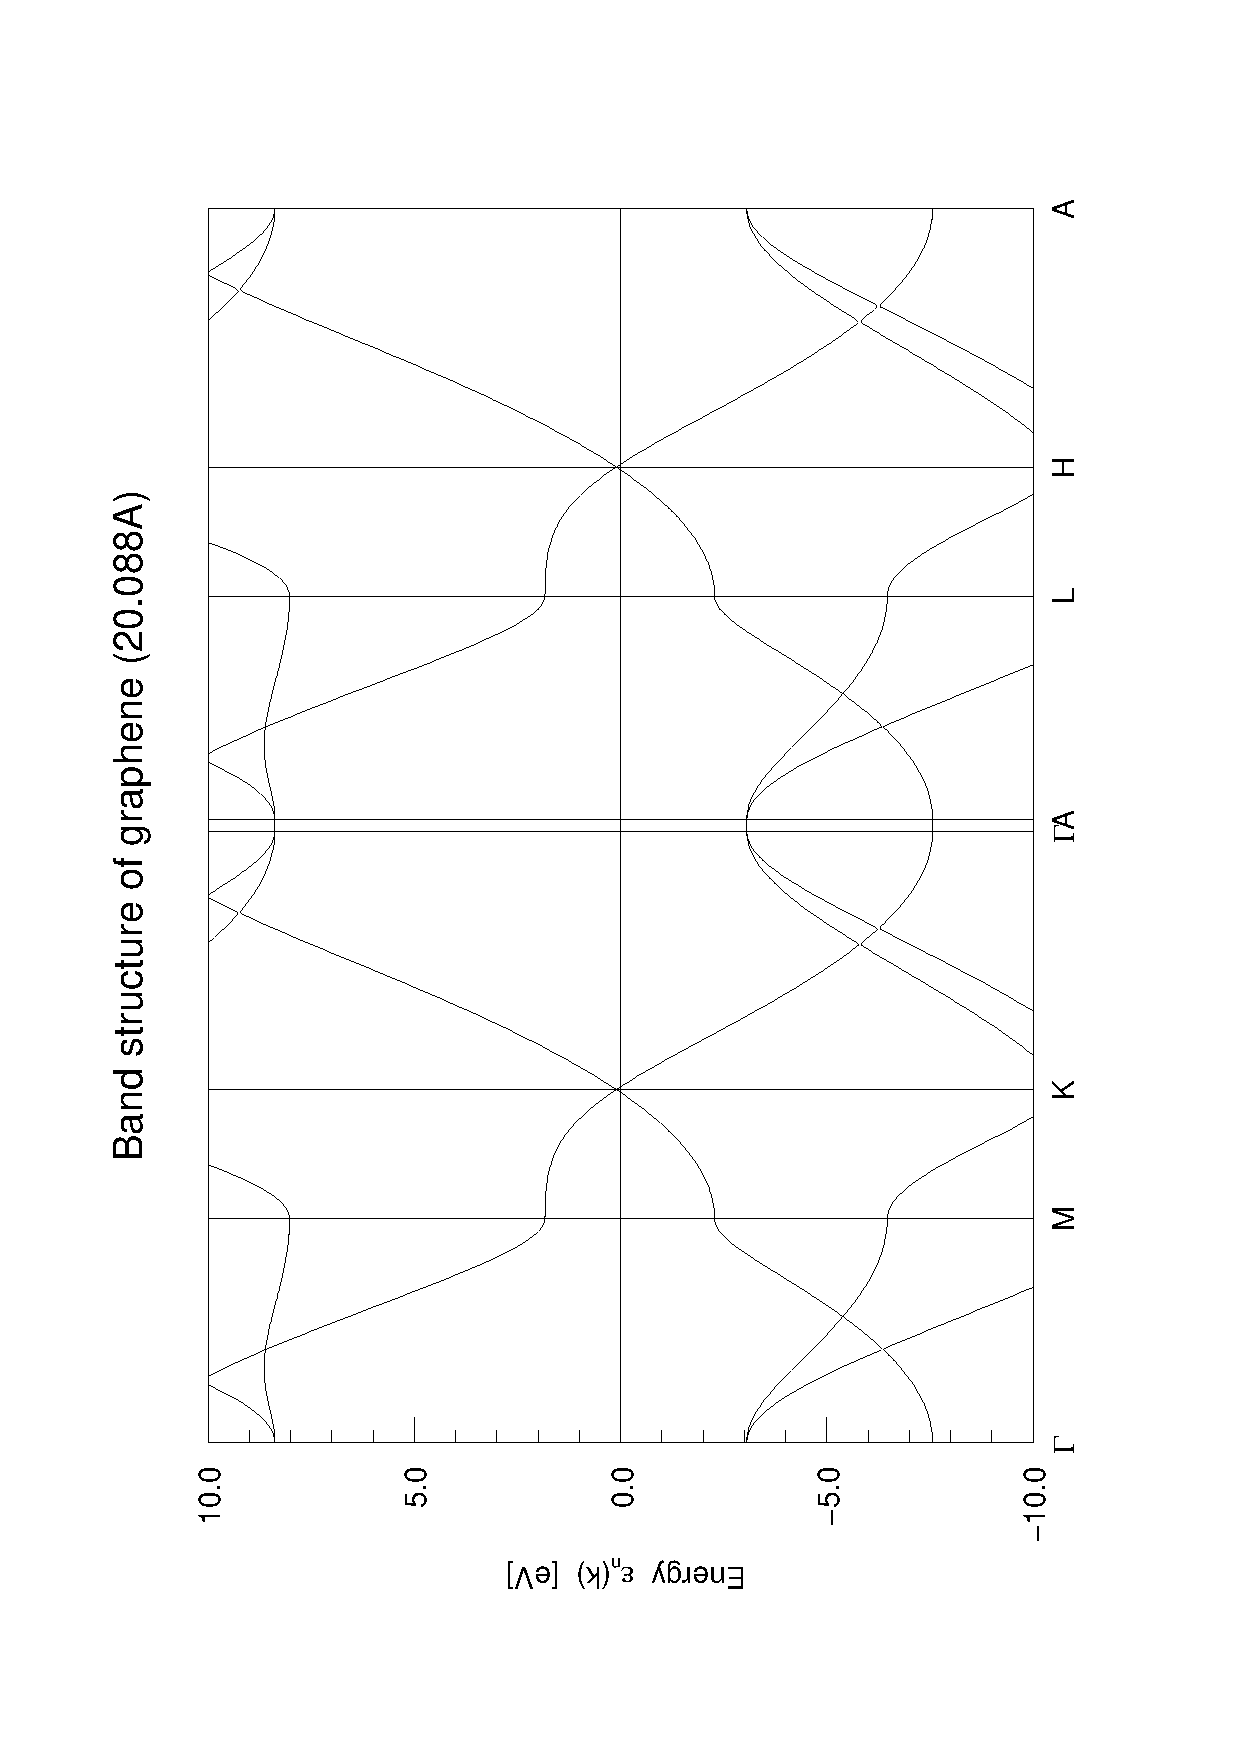
\includegraphics[width=\textwidth]{Results/Graphene/Graphene20A/graphene20Aband.pdf}
					\end{minipage}
					\begin{minipage}[t]{\textwidth}
						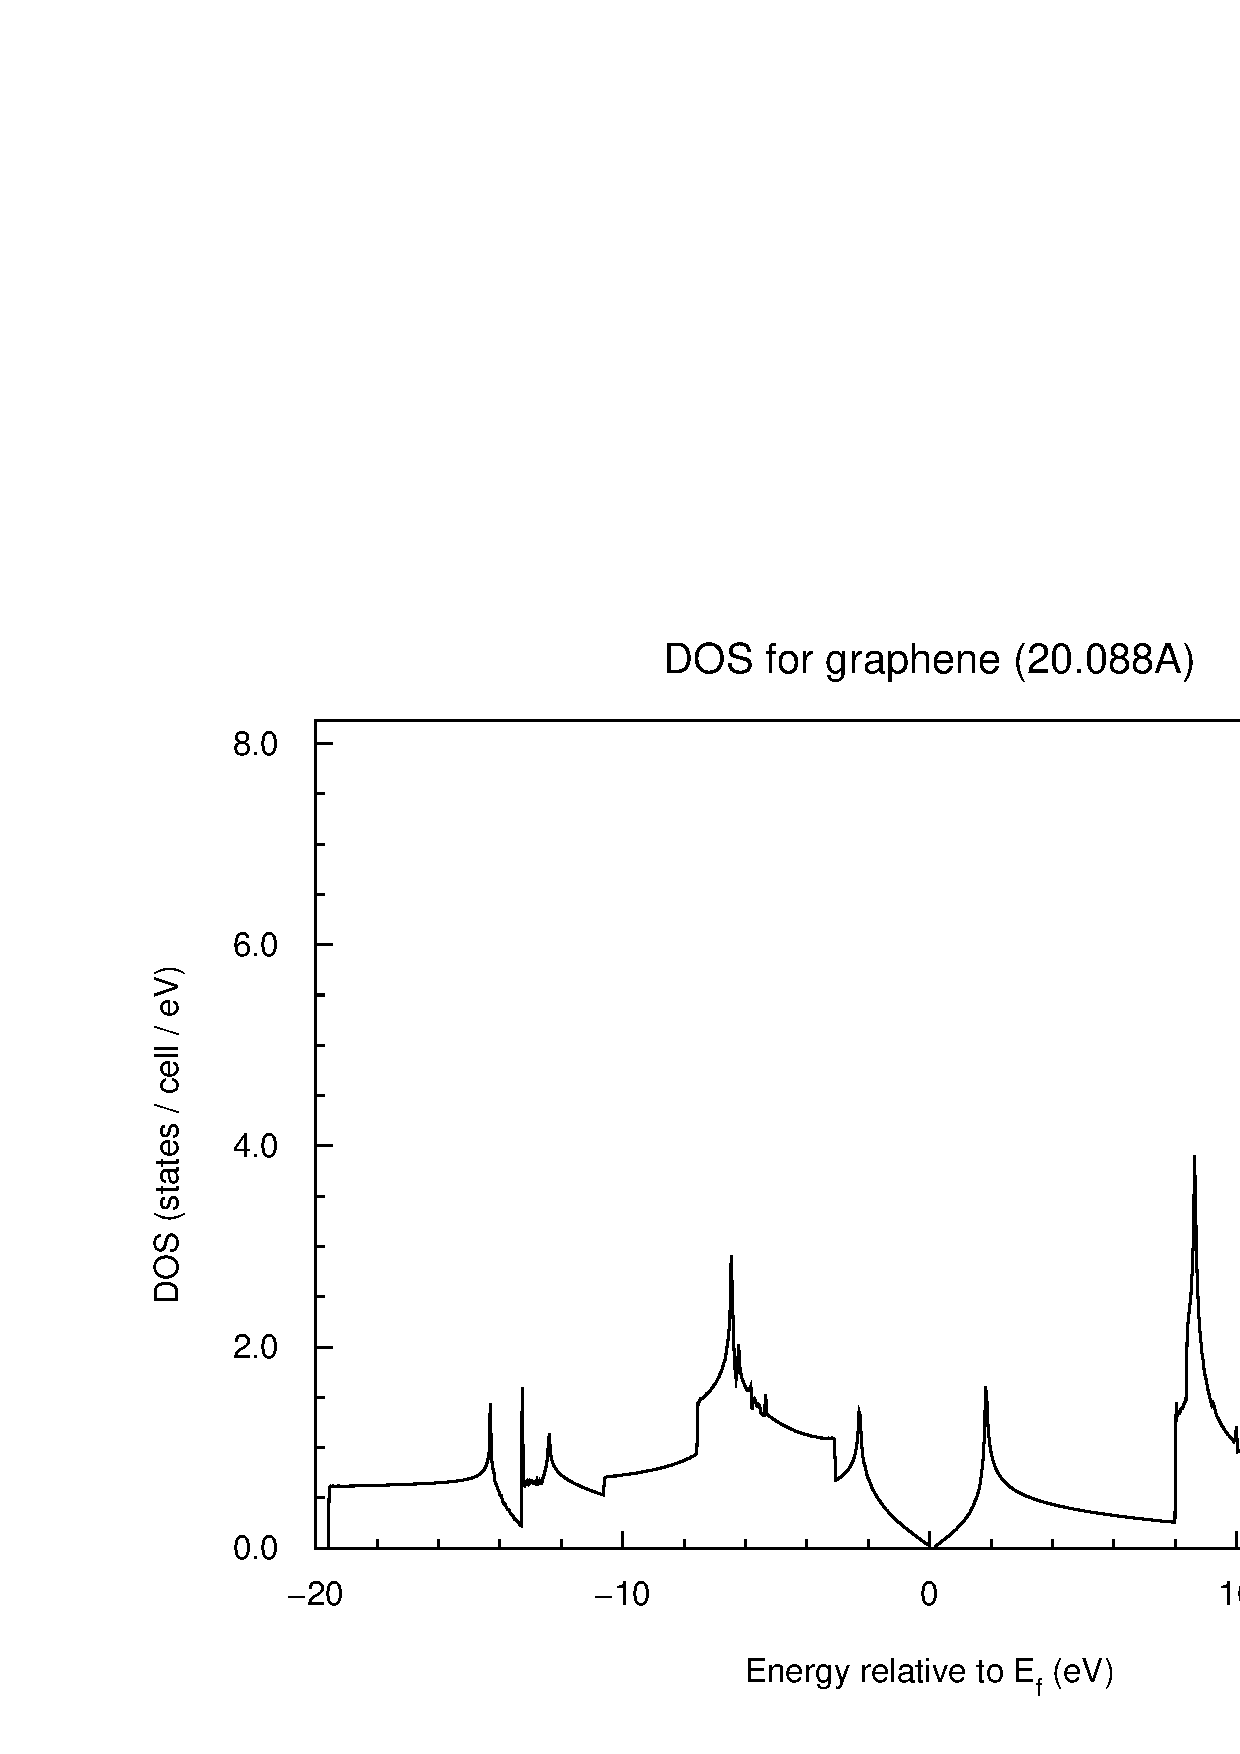
\includegraphics[width=\textwidth]{Results/Graphene/Graphene20A/graphene20Ados.pdf}
					\end{minipage}
					\caption{Band structure and total density of states of graphene (20 $\AA$, FPLO $100\times100\times4$).}
					\label{fig:GrapheneProperties}
				\end{figure}
				\begin{figure}
					\begin{minipage}[t]{\textwidth}
						\includegraphics[width=\textwidth]{Results/Graphene/Graphene20A/graphene20APi.pdf}
					\end{minipage}
					\begin{minipage}[t]{\textwidth}
						\includegraphics[width=\textwidth]{Results/Graphene/Graphene20A/graphene20ASigma.pdf}
					\end{minipage}
					\caption{Weighted band structure of graphene. \textbf{Top:} weighted $\pi$ bands. \textbf{Bottom:} weighted 2s, $2p_x$ and $2p_y$ orbitals. (20 $\AA$, FPLO $100\times100\times4$)}
					\label{fig:GraphenePiSigma}
				\end{figure}
				\begin{figure}
					\includegraphics[width=\textwidth]{Results/Graphene/Graphene20A/graphene20AdosPiSigma.pdf}
					\caption{DOS for the p and sigma-orbitals of graphene with a physically incorrect negative DOS at approximately 18.3 eV (FPLO $100\times100\times4$).}
					\label{fig:GraphenePiSigmaDos}
				\end{figure}				
				Graphene has a total energy of \textbf{-76.168} Ha and three \textbf{sigma} orbitals (2s hybridized with 2p, plotted in Figure \ref{fig:GraphenePiSigma}, bottom), responsible for the planar carbon-carbon bondings and one \textbf{$\pi$} orbital (Figure \ref{fig:GraphenePiSigma}, top). For a whole lattice the $\pi$ orbitals merge and can be seen as delocalized electrons, that are one reason for the copper-equivalent conductivity properties. The contribution of the p and s-orbitals are displayed in Figure \ref{fig:GraphenePiSigmaDos}. We have to mention, that only the $p_z$ orbital contributes to the DOS in the area around the Fermi level. Moreover graphene is a \textbf{zero-gap semiconductor}, i.e. that at the Fermi energy of 0 eV there are no states (Figure \ref{fig:GrapheneProperties}, bottom) and the band-gap is 0 eV. In the band structure (Figure \ref{fig:GrapheneProperties}, top) we find at the K point a 0 eV energy gap, which represents the zero-gap mentioned before and is called \textbf{Dirac point}. At the Dirac point the energy dispersion is linear, which leads to fermions behaving like relativistic particles, described by the Dirac equation near the Dirac point. \\\\
				Before continuing with the modification of graphene we have noticed, that in almost every our DOS plots are physically incorrect negative values. This could be solved by extending the FPLO basis. As a cause we will limited our discussions of areas without significant influence of negative density  of states (Figure \ref{fig:GraphenePiSigmaDos}).
	
			\subsection{Boron-modified graphene}
				\begin{figure}
					\begin{minipage}[t]{\textwidth}
						\includegraphics[width=\textwidth]{Results/Bor/Bor1R/dos.pdf}
					\end{minipage}
					\begin{minipage}[t]{\textwidth}
						\includegraphics[width=\textwidth]{Results/Graphene/GrapheneNew/dos.pdf}
					\end{minipage}		
					\caption{Comparison DOS between boron modified graphene (\textbf{top}, FPLO $20\times20\times20$) and graphene (\textbf{bottom}, FPLO $100\times100\times20$).}
					\label{fig:GrapheneBorDOSComparisson}
				\end{figure}
				\begin{figure}
					\begin{minipage}[t]{\textwidth}
						\includegraphics[width=\textwidth]{Results/Bor/Bor1R/bweights.pdf}
					\end{minipage}
					\begin{minipage}[t]{\textwidth}
						\includegraphics[width=\textwidth]{Results/Graphene/GrapheneNew/bweights.pdf}
					\end{minipage}
					\caption{Comparison of the weighted band structures between boron modified graphene (\textbf{top}, FPLO $20\times20\times20$) and graphene (\textbf{bottom}, FPLO $100\times100\times20$). }
					\label{fig:GrapheneBorBweightsComparisson}
				\end{figure}
				In this section we will discuss the results obtained by different amounts of boron impurities in a graphene lattice. We studied the graphene compound with 50\% of boron impurities. \\\\
				Boron has one valence electron less than carbon and it should therefore lead to an acceptor-intercalated graphene, which means it should increase the electronic conductivity. Regarding the DOS comparison (Figure \ref{fig:GrapheneBorDOSComparisson}) we can conclude that there are more states after the Fermi level in the boron doped lattice, consequently the boron bulk is \textbf{metallic} and the conductivity should be increased. Nevertheless behind the Fermi level opened a gap of approximately 2.6 eV in the DOS, which could limit the conducting properties of the graphene compound. Considering the band structures (Figure \ref{fig:GrapheneBorBweightsComparisson}), we observe the a loss of the Dirac point due to the loss of symmetry. \\\\
				For finding information about the stablest form we tried a relaxation of the given BC mono layer with the FPLO force module, which could not be calculated due too small forces. Therefore we relaxed the lattices manually by fitting the total energy. The only degree of freedom is the lattice parameter in the x and y plane for which we will optimize the total energy. The distance fit (\ref{fig:boronFitting}) yields a optimal parameter of \textbf{2.687} $\boldsymbol{\AA}$ with a total energy of \textbf{-62.881 Ha}.
				\begin{figure}
					\includegraphics[width=\textwidth]{Results/Bor/Bor1R/data.pdf}
					\caption{Distance fitting of $C_{1-x}B_x,x= 1 / 2$.}
					\label{fig:boronFitting}
				\end{figure}
			
			\subsection{Nitrogen modified graphene}
				\begin{figure}
					\begin{minipage}[t]{\textwidth}
						\includegraphics[width=\textwidth]{Results/Nitrogen/Nitrogen1R/bweights.pdf}
					\end{minipage}
					\begin{minipage}[t]{\textwidth}
						\includegraphics[width=\textwidth]{Results/Graphene/GrapheneNew/bweights.pdf}
					\end{minipage}
					\caption{Comparison of the weighted band structures between nitrogen modified graphene (\textbf{top}, FPLO $20\times20\times20$) and graphene (\textbf{bottom}, FPLO $100\times100\times20$).}
					\label{fig:GrapheneNitrogenComparisson}
				\end{figure}
				\begin{figure}
					\begin{minipage}[t]{\textwidth}
						\includegraphics[width=\textwidth]{Results/Nitrogen/Nitrogen1R/dos.pdf}
					\end{minipage}
					\begin{minipage}[t]{\textwidth}
						\includegraphics[width=\textwidth]{Results/Graphene/GrapheneNew/dos.pdf}
					\end{minipage}											
					\caption{Comparison DOS between nitrogen modified graphene (\textbf{top}, FPLO $20\times20\times20$) and graphene (\textbf{bottom}, FPLO $100\times100\times20$).}
					\label{fig:GrapheneNitrogenDOSComparisson}
				\end{figure}
				Having obtained results for boron-doped graphene we want to continue with observing a CN mono-layer. \\\\
				Nitrogen has one valence electron more than carbon and it should therefore lead to a donator-inercalated graphene lattice. As in the boron-carbon compound there are more states near the Fermi level, which implies an improved conductivity. Moreover NC also has a band-gap between -2.6 eV and 7.3 eV. Moreover the NC layer also loses its Dirac point, apparent to the loss of symmetry. \\\\
				\begin{figure}
					\includegraphics[width=\textwidth]{Results/Nitrogen/Nitrogen1R/data.pdf}
					\caption{Unite cell length fit of $C_{1-x}B_x,x= 1 / 2$.}
					\label{fig:nitrogenFitting}
				\end{figure}
				As in Boron doped graphene we now want to focus on the relax the NC compound. Therefore we fitted the energy of different distances (Figure \ref{fig:nitrogenFitting}) and found a minimum at a distance of \textbf{2.477} $\boldsymbol{\AA}$ with an energy of \textbf{-92.743 Ha}.
				
			\subsection{Silicon modified graphene}
				\begin{figure}
					\begin{minipage}[t]{\textwidth}
						\includegraphics[width=\textwidth]{Results/Silicon/Silicon1R/bweights.pdf}
					\end{minipage}
					\begin{minipage}[t]{\textwidth}
						\includegraphics[width=\textwidth]{Results/Graphene/GrapheneNew/bweights.pdf}
					\end{minipage}	
					\caption{Comparison of the weighted band structures between silicon modified graphene (\textbf{top}, FPLO $20\times20\times20$) and graphene (\textbf{bottom}, FPLO $100\times100\times20$).}
					\label{fig:GrapheneSiliconComparisson}
				\end{figure}
				\begin{figure}
					\begin{minipage}[t]{\textwidth}
						\includegraphics[width=\textwidth]{Results/Silicon/Silicon1R/dos.pdf}
					\end{minipage}
					\begin{minipage}[t]{\textwidth}
						\includegraphics[width=\textwidth]{Results/Graphene/GrapheneNew/dos.pdf}
					\end{minipage}											
					\caption{Comparison DOS between silicon modified graphene (\textbf{top}, FPLO $20\times20\times20$) and graphene (\textbf{bottom}, FPLO $100\times100\times20$).}
					\label{fig:GrapheneSiliconDOSComparisson}
				\end{figure}
				The last material we want to observe is silicon doped graphene. Silicon is in the same group as carbon, i.e. its count of valence electrons is equal to carbon. On he other hand it is located in the next period hence it has plenty more electrons and a bigger atomic radius than boron or nitrogen. Due to the many electrons the Fermi level and the orbitals previously responsible for the electronic properties changed from 2s and 2p to 3s and 3p (Figure \ref{fig:GrapheneSiliconComparisson}). In Addition the SC mono layer has a band gap of approximated 2 eV and is therefore a semiconductor. Nevertheless it has a very high state of density right before the Fermi level. \\\\
				\begin{figure}
					\includegraphics[width=\textwidth]{Results/Silicon/Silicon1R/data.pdf}
					\caption{Distance fitting of $C_{1-x}B_x,x= 1 / 2$.}
					\label{fig:siliconFitting}
				\end{figure}
				For a observation of the stability we found the energetic minimum at a unit cell length of \textbf{3.112} $\boldsymbol{\AA}$, which leads to the biggest unit cell size of all three compounds, caused presumable due to the huge atom radius of silicon ($\approx 111$ pm).
				In Addition the total energy of the silicon compound is very different to the total energy of nitrogen or boron with a value of \textbf{-327.459 eV}.
				\begin{table}[H]
					\centering
					\begin{tabular}{cccc}
						\midrule
						C & B & N & Si \\
						\midrule 
						-76.168 eV & -62.881 Ha & -92.743 Ha & -327.459 Ha \\
						\bottomrule
					\end{tabular}
					\caption{Comparison of the total energy's for graphene and graphene modified with boron, nitrogen or silicon.}
				\end{table}
				\begin{table}[H]
					\centering
					\begin{tabular}{cccc}
						\midrule
						C & B & N & Si \\
						\midrule 
						2.456 $\AA$ & 2.687 $\AA$ & 2.477 $\AA$ & 3.112 $\AA$ \\
						\bottomrule
					\end{tabular}
					\caption{Comparison of graphene and the relaxed unite cell lengths.}
				\end{table}				
				For the purpose of completeness we added band structures and density of states of different modifications and doping densities (see Figures \ref{fig:BoronDensityComparisson}, \ref{fig:NitrogenDensityComparisson}, \ref{fig:SiliconDensityComparisson}, \ref{fig:BoronDOSDensityComparisson}, \ref{fig:NitrogenDOSComparisson}, \ref{fig:SiliconDOSComparisson}). From the figures we can obtain, that the number of bands rise with the size of the unite cell, caused by the number of unequal atoms, having different orbitals. Furthermore we obtain for a reducing density a rising graphene character by comparing the density of states.
				\begin{figure}
					\begin{minipage}[t]{0.9\textwidth}
						\includegraphics[width=\textwidth]{Results/Bor/Bor1/bor1band.pdf}
					\end{minipage}
					\begin{minipage}[t]{0.9\textwidth}
						\includegraphics[width=\textwidth]{Results/Bor/Bor5/bor5band.pdf}
					\end{minipage}
					\begin{minipage}[t]{0.3\textwidth}
						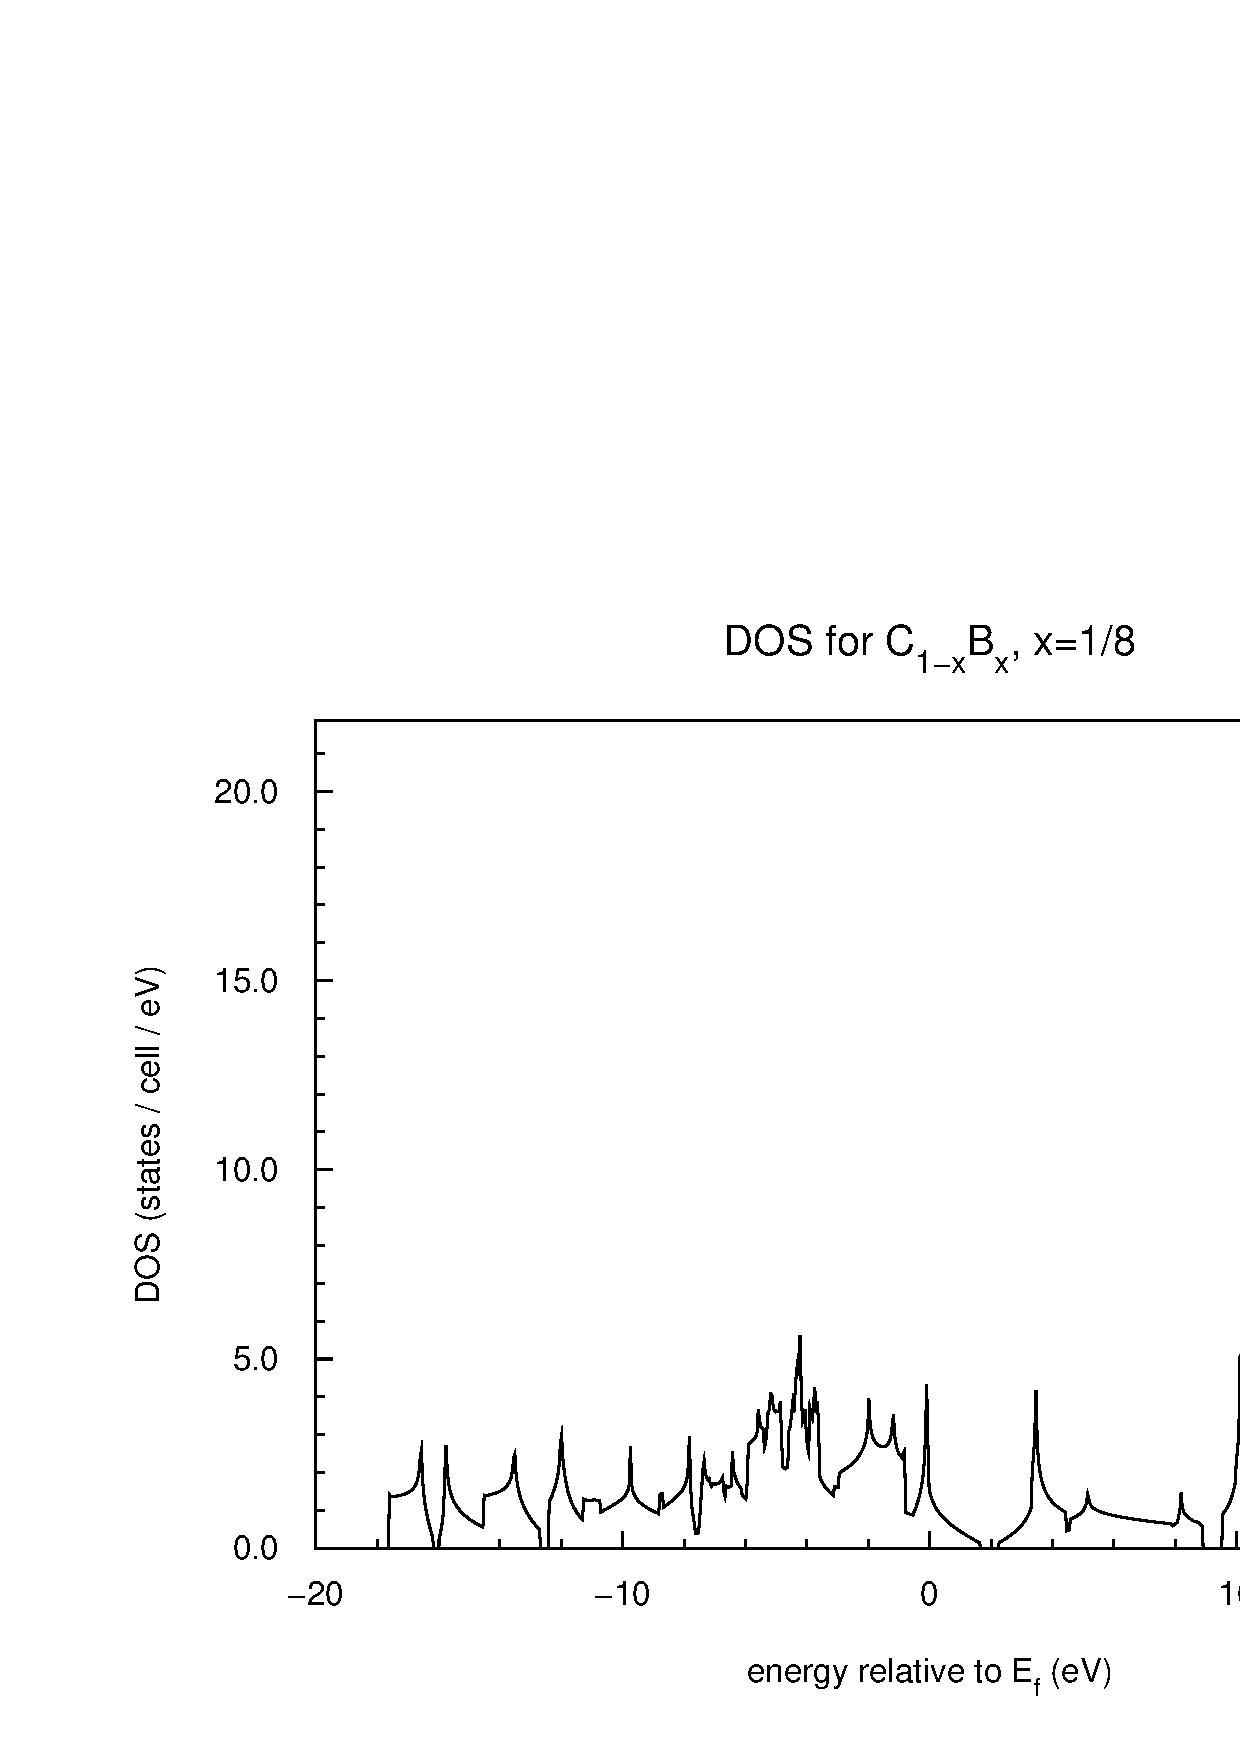
\includegraphics[width=\textwidth]{Results/Bor/Bor2/bor2band.pdf}
					\end{minipage}
					\begin{minipage}[t]{0.3\textwidth}
						\includegraphics[width=\textwidth]{Results/Bor/Bor3/bor3band.pdf}
					\end{minipage}
					\begin{minipage}[t]{0.3\textwidth}
						\includegraphics[width=\textwidth]{Results/Bor/Bor4/bor4band.pdf}
					\end{minipage}															
					\caption{Comparison of the band structures from boron-modified graphene with different densities (FPLO $100x100x4$).}
					\label{fig:BoronDensityComparisson}
				\end{figure}				
				\begin{figure}
					\begin{minipage}[t]{0.9\textwidth}
						\includegraphics[width=\textwidth]{Results/Nitrogen/Nitrogen1/nitrogen1band.pdf}
					\end{minipage}
					\begin{minipage}[t]{0.9\textwidth}
						\includegraphics[width=\textwidth]{Results/Nitrogen/Nitrogen5/nitrogen5band.pdf}
					\end{minipage}
					\begin{minipage}[t]{0.3\textwidth}
						\includegraphics[width=\textwidth]{Results/Nitrogen/Nitrogen2/nitrogen2band.pdf}
					\end{minipage}
					\begin{minipage}[t]{0.3\textwidth}
						\includegraphics[width=\textwidth]{Results/Nitrogen/Nitrogen3/nitrogen3band.pdf}
					\end{minipage}
					\begin{minipage}[t]{0.3\textwidth}
						\includegraphics[width=\textwidth]{Results/Nitrogen/Nitrogen4/nitrogen4band.pdf}
					\end{minipage}															
					\caption{Comparison of the band structures from nitrogen-modified graphene with different densities (FPLO $100x100x4$)}
					\label{fig:NitrogenDensityComparisson}
				\end{figure}
				\begin{figure}
					\begin{minipage}[t]{0.9\textwidth}
						\includegraphics[width=\textwidth]{Results/Silicon/Silicon1/silicon1band.pdf}
					\end{minipage}
					\begin{minipage}[t]{0.9\textwidth}

						\includegraphics[width=\textwidth]{Results/Silicon/Silicon5/silicon5band.pdf}
					\end{minipage}
					\begin{minipage}[t]{0.3\textwidth}
						\includegraphics[width=\textwidth]{Results/Silicon/Silicon2/silicon2band.pdf}
					\end{minipage}
					\begin{minipage}[t]{0.3\textwidth}
						\includegraphics[width=\textwidth]{Results/Silicon/Silicon3/silicon3band.pdf}
					\end{minipage}
					\begin{minipage}[t]{0.3\textwidth}
						\includegraphics[width=\textwidth]{Results/Silicon/Silicon4/silicon4band.pdf}
					\end{minipage}															
					\caption{Comparison of the band structures from silicon-modified graphene with different densities (FPLO $100x100x4$)}
					\label{fig:SiliconDensityComparisson}
				\end{figure}
				\begin{figure}
					\begin{minipage}[t]{0.9\textwidth}
						\includegraphics[width=\textwidth]{Results/Bor/Bor1/bor1dos.pdf}
					\end{minipage}
					\begin{minipage}[t]{0.9\textwidth}
						\includegraphics[width=\textwidth]{Results/Bor/Bor5/bor5dos.pdf}
					\end{minipage}
					\begin{minipage}[t]{0.3\textwidth}
						\includegraphics[width=\textwidth]{Results/Bor/Bor2/bor2dos.pdf}
					\end{minipage}
					\begin{minipage}[t]{0.3\textwidth}
						\includegraphics[width=\textwidth]{Results/Bor/Bor3/bor3dos.pdf}
					\end{minipage}
					\begin{minipage}[t]{0.3\textwidth}
						\includegraphics[width=\textwidth]{Results/Bor/Bor4/bor4dos.pdf}
					\end{minipage}															
					\caption{Comparison of the DOS from boron-modified graphene with different densities (FPLO $100x100x4$)}
					\label{fig:BoronDOSDensityComparisson}
				\end{figure}				
				\begin{figure}
					\begin{minipage}[t]{0.9\textwidth}
						\includegraphics[width=\textwidth]{Results/Nitrogen/Nitrogen1/nitrogen1dos.pdf}
					\end{minipage}
					\begin{minipage}[t]{0.9\textwidth}
						\includegraphics[width=\textwidth]{Results/Nitrogen/Nitrogen5/nitrogen5dos.pdf}
					\end{minipage}
					\begin{minipage}[t]{0.3\textwidth}
						\includegraphics[width=\textwidth]{Results/Nitrogen/Nitrogen2/nitrogen2dos.pdf}
					\end{minipage}
					\begin{minipage}[t]{0.3\textwidth}
						\includegraphics[width=\textwidth]{Results/Nitrogen/Nitrogen3/nitrogen3dos.pdf}
					\end{minipage}
					\begin{minipage}[t]{0.3\textwidth}
						\includegraphics[width=\textwidth]{Results/Nitrogen/Nitrogen4/nitrogen4dos.pdf}
					\end{minipage}															
					\caption{Comparison of the DOS from nitrogen-modified graphene with different densities (FPLO $100x100x4$)}
					\label{fig:NitrogenDOSComparisson}
				\end{figure}
				\begin{figure}
					\begin{minipage}[t]{0.9\textwidth}
						\includegraphics[width=\textwidth]{Results/Silicon/Silicon1/silicon1dos.pdf}
					\end{minipage}
					\begin{minipage}[t]{0.9\textwidth}
						\includegraphics[width=\textwidth]{Results/Silicon/Silicon5/silicon5dos.pdf}
					\end{minipage}
					\begin{minipage}[t]{0.3\textwidth}
						\includegraphics[width=\textwidth]{Results/Silicon/Silicon2/silicon2dos.pdf}
					\end{minipage}
					\begin{minipage}[t]{0.3\textwidth}
						\includegraphics[width=\textwidth]{Results/Silicon/Silicon3/silicon3dos.pdf}
					\end{minipage}
					\begin{minipage}[t]{0.3\textwidth}
						\includegraphics[width=\textwidth]{Results/Silicon/Silicon4/silicon4dos.pdf}
					\end{minipage}															
					\caption{Comparison of the DOS from silicon-modified graphene with different densities (FPLO $100x100x4$)}
					\label{fig:SiliconDOSComparisson}
				\end{figure}
				
				
					
				
				

				
			
	
	
			
		
		
		
			
		
		
		
		
		
		
		
			 
		
		

		
	\chapter{Tight binding model}
	For electrons in a periodical lattice that are strongly bound to positive ions, as for lower orbital ones, we can use the tight binding model to calculate the band structure. \\
	We will start with a general derivation of the tight binding approximation and finish with an analytical solution of the nearest neighbor tight binding of graphene.
		
	\section{Tight binding model}
		The one electron Hamiltonian labeled by l is given by
		\begin{equation}
			\hat H_l = - \frac{\hbar^2}{2m_e} \nabla_l^2 + \sum_{j=1}{N}(\vec{r_l - R_j}),
		\end{equation}
		where we are regarding a Bravais lattice, with positive ions on the positions $\vec{R_j}$ and N as number of lattice sites. The Hamiltonian of all electrons is therefore given by : 
		\begin{equation}
			\hat H = \sum_{j=1}^{N} \hat H_l.
		\end{equation}
		In the \textit{tight binding model} each electron is "tightly" bound to a particular lattice site and can be described by
		\begin{equation}
			\hat H_l^a = - \frac{\hbar^2}{2m_e} \nabla_l^2 + V(\vec{r_l - R_l}).
		\end{equation}
		In addition we define the potential energy as $\Delta V = \sum_{j \neq l}^N V(\vec{r_l - R_j})$ from the other ions at sites $\vec{R_j}, j \neq l$, which can be treated pertubatively. While calculating the band structure of a lattice with more than one atom per unit cell (as for example of graphene) we need to notice that translating the sub-lattice A into B is not a symmetry operation. As a consequence we have to treat the different sub-lattices apart by linearizing the trial wave-function. For two atoms per unit cell, like in the honeycomb lattice from graphene, we may write down the trial wave-function as :
		\begin{equation}
			\label{eq:tightBindingPsiSum}
			\psi_\vec k (\vec{r}) = a_\vec k  \psi_\vec k^{(A)} (\vec r) + b_\vec k \psi_\vec k^{(B)}(\vec r),
		\end{equation}
		where A and B represent the sub-lattices and $a_\vec k$ and $b_\vec k$ are complex functions of $\vec k$. $\psi_\vec k^{(A)}$ and $\psi_\vec k^{(B)}$ are Bloch functions and may be written as : 
		\begin{equation}
			\label{eq:tightBindingBlochWave}
			\psi_\vec k^{(j)}(\vec r) = \sum_{\vec R_l} e^{i \vec{k \cdot R_l}} \phi^{(j)}(\vec{r} + \boldsymbol{\delta_j} - \vec{R_l})
		\end{equation}
		with $\delta_j$ as vector connecting the two sub-lattices. For a better understanding we shortly want to prove the Bloch compatibility of the last relation
		\begin{equation}
			\begin{split}
				\psi(\vec{r + R}) &= \sum{R_l} e^{i \vec{k \cdot R_l}} \phi(\vec{r + R} + \boldsymbol{\delta_j} - \vec{R_l}) \\
				&=  e^{i \vec{k \cdot R}}\sum{R_l} e^{i \vec{k \cdot R_l - R}} \phi(\vec{r} + \boldsymbol{\delta_j} - (\vec{R_l - R} )) \\
				&= e^{i \vec{k \cdot R}}\sum{R_l} e^{i \vec{k \cdot R'}} \phi(\vec{r} + \boldsymbol{\delta_j} - \vec{R'} ) \\
				&= e^{i \vec{k \cdot R}} \psi(\vec r + \boldsymbol \delta_j).
			\end{split}				
		\end{equation}
		The next aim is to find a general solution for the Schrödinger equation
		\begin{equation}
			\hat H | \psi_\vec k \rangle = \epsilon_\vec k | \psi_\vec k \rangle
		\end{equation}
		of the tight binding model. Multiplying the above equation by $\langle \psi_\vec k^* |$ yields
		\begin{equation}
			\langle \psi_\vec k^* | \hat H | \psi_\vec k \rangle = \epsilon_\vec k \langle \psi_\vec k | \psi_\vec k \rangle,
		\end{equation}
		which can be rewritten in matrix form with the help of Eq. \ref{eq:tightBindingPsiSum}.
		\begin{equation}
			\begin{pmatrix}
				a_\vec k^* & b_\vec k^*
			\end{pmatrix}
			 H_\vec k 
			 \begin{pmatrix}
				a_\vec k \\
				b_\vec k
			 \end{pmatrix}
			 = \epsilon_\vec k 
			 \begin{pmatrix}
				a_\vec k^* & b_\vec k^*
			 \end{pmatrix}
			  S_\vec k 
			 \begin{pmatrix}
			 	a_\vec k \\
				b_\vec k
			\end{pmatrix}
		\end{equation}
		with the Hamiltonian matrix defined as
		\begin{equation}
			H_\vec k \equiv 
			\begin{pmatrix}
				\psi_\vec k^{(A)*} \hat H \psi_\vec k^{(A)} & \psi_\vec k^{(A)*} \hat H \psi_\vec k^{(B)} \\
				\psi_\vec k^{(B)*} \hat H \psi_\vec k^{(A)} & \psi_\vec k^{(B)*} \hat H \psi_\vec k^{(B)}
			\end{pmatrix}
			= H_\vec k^\dagger
		\end{equation}
		and the overlap matrix
		\begin{equation}	  
			S_\vec k \equiv 
			\begin{pmatrix}
				\psi_\vec k^{(A)*} \psi_\vec k^{(A)} & \psi_\vec k^{(A)*} \psi_\vec k^{(B)} \\
				\psi_\vec k^{(B)*} \psi_\vec k^{(A)} & \psi_\vec k^{(B)*} \psi_\vec k^{(B)}
			\end{pmatrix}
			= S_\vec k^\dagger,
		\end{equation}
		that needs to be included because of the non orthogonality of the wave function $\psi_\vec k$. The eigenfunctions can now be obtained by the secular equation :
		\begin{equation}
			det[H_\vec k - \epsilon_\vec k^\lambda S_\vec k] = 0
		\end{equation}
		With help of Eq. \ref{eq:tightBindingBlochWave} we can rewrite the matrix entries of the Hamiltonian matrix into
		\begin{align}
			\label{eq:tightHij}
			H_\vec k^{ij} &= \sum_{\vec{R_l, R_m}} e^{i \vec{k \cdot (\vec{R_l - R_m)}}} \int d^2 r \phi^{(i)*}(\vec{r } + \boldsymbol{\delta_i} - \vec{R_l}) H \phi^{(j)}(\vec{r} + \boldsymbol{\delta_i} - \vec{R_m}) \\
			&= N \sum_{\vec R_l} e^{i \vec{k \cdot R_l}} \int d^2 \phi^{(i)*}(\vec r)[H^a + \Delta V] \phi^{(j)}(\vec{r} + \boldsymbol{\delta_{ij}} - \vec{R_l}) \\
			&= N (\epsilon^{(i)} s_\vec k^{ij} + t_\vec k^{ij}),
		\end{align}
		where $\delta_{ij} \equiv \delta_j - \delta_i$,
		\begin{equation}
			\label{eq:tightSij}
			s_\vec k^{ij} \equiv \sum_{\vec R_l} e^{i \vec{k \cdot R_l}} \int d^2 r \phi^{(i)*}(\vec{r} + \boldsymbol{\delta_i} - \vec{R_k}) \phi^{(j)}(\vec{r} + \boldsymbol{\delta_j} - \vec{R_mk}) = \frac{S_k^{ij}}{N}
		\end{equation}
		and the so called hopping matrix is defined as
		\begin{equation}
			t_\vec k^{ij} = \sum_{\vec R_l} e^{i \vec{k \cdot R_l}} \int d^2 r \phi^{(i)*}(\vec{r} + \boldsymbol{\delta_i} - \vec{R_k}) \Delta V \phi^{(j)}(\vec{r} + \boldsymbol{\delta_j} - \vec{R_m})
		\end{equation}
		The secular equation now reads :
		\begin{equation}
			\label{eq:generalTightBindingSolution}
			det[t_\vec k^{ij} - \epsilon_\vec k ^\lambda - \epsilon^{(i)}] = 0
		\end{equation}
		All of the atoms on the different sub-lattices have the same electronic configuration ($p_z$ orbitals) and therefore $\epsilon^{(i)} = \epsilon_0$ becomes a constant, which we will omit in future discussions.
					
	\section{Nearest neighbor tight binding for graphene}
		\begin{figure}[h]
			\centering
			\includegraphics[width=0.5\textwidth]{figures/TightBinding/tightBinding.png}
			\caption{Nearest (nn) and Next nearest neighbors (nnn) of a carbon atom in the hexagonal lattice.$\vec R_1$, $\vec R_2$ and $\vec R_3$ connect the centered lattice site to its next nearest neighbors. $\boldsymbol{\delta_3}$ is the connection vector between the A and the B sublattice. The nearest neighbor vectors can be build from the next nearest neighbor vectors.}
			\label{fig:tighBindingHoneycomb}
		\end{figure}
		Having found a general solution, we continue deriving a specific one for graphene with its honeycomb lattice. The connection vectors to the next nearest and the nearest neighbor are given in Fig: \ref{fig:tighBindingHoneycomb}.
		\begin{align}
			\label{eq:tightBindingVectors}
			\vec R_1 = \frac{a}{2} 
			\begin{pmatrix} 
				\sqrt{3} \\
			 	3
			 \end{pmatrix} & 
			 \vec R_2 = \frac{a}{2} 
			 \begin{pmatrix} 
			 	3 \\
			 	- \sqrt{3}
			 \end{pmatrix}
			 \vec R_3 = a 
			 \begin{pmatrix} 
			 	\sqrt{3} \\ 
			 	0
			 \end{pmatrix} &
			 \boldsymbol{\delta_3} = a \begin{pmatrix} 0 \\ -1\end{pmatrix}
		\end{align}
		We start with the secular equation (\ref{eq:generalTightBindingSolution}) and neglect the energy shift $\epsilon_0$, which only contains a shift in the energy.
		\begin{equation}
			\begin{pmatrix}
				H_k^{AA} - \epsilon s_k^{AA} & 	H_k^{AB} - \epsilon s_k^{AB} \\
				H^{BA} - \epsilon s_k^{BA} & 	H_k^{BB} - \epsilon s_k^{BB}
			\end{pmatrix}
		\end{equation}
		With the given variables $H^{ij}$ and $S^{ij}$. Equation \ref{eq:tightHij} can be rewritten under the graphene double sub-lattice conditions as:
		\begin{equation}
			H_k^{ij} = t_k^{ij}
		\end{equation}
		The N cancels from the sum over the lattice sites and $\epsilon^{(i)}$ is omitted. In addition on can write: 
		\begin{equation}
			\begin{split}
				H_k^{AA} = t_k^{AA} &= \sum_{\vec R_1}^{\vec R_l} e^{i \vec{k \cdot R_l}} \underbrace{\int d^2 r \phi^{(A)*}(\vec{r}) \Delta V \phi^{(A)}(\vec{r} + \boldsymbol{\delta_3}}_{t_{nnn}} \\ 
				 &= t_{nnn} (e^{i \vec{k \cdot R_1}} + e^{-i \vec{k \cdot R_1}} + e^{i \vec{k \cdot R_2}} + e^{-i \vec{k \cdot R_2}} + e^{i \vec{k \cdot R_3}} + e^{-i \vec{k \cdot R_3}}) \\
				 &= 2t_{nnn} ( \sum_{i=1}^{3} cos(\vec{k \cdot R_i}))	= t_k^{BB}
			\end{split}			
		\end{equation}
		\begin{equation}
			\begin{split}		
				H_k^{AB} = t_k^{AB} &= \sum_{\vec R_1}^{\vec R_3} e^{i \vec{k \cdot R_l}} \underbrace{\int d^2 r \phi^{(A)*}(\vec{r}) \Delta V \phi^{(B)}(\vec{r} + \boldsymbol{\delta_j})}_{t} \\
				&= t(1 + e^{i \vec{-k \cdot \vec{R_1}} + e^{-i \vec{k \cdot R_3}}}) 	\\
				&= (t_k^{BA})^*	
			\end{split}			
		\end{equation}
		Eq. \ref{eq:tightSij} can now be transformed to
		\begin{equation}
				s_k^{AA} = s_k^{BB} = 1	
		\end{equation}
		due to the normalizations of the atomic wave-functions ($\int d^2 r \phi^{(j)*}(\vec r) \Delta V \phi^{(j)}(\vec r) = 1$) we have
		\begin{equation}
			\begin{split}
				s_k^{AB} &= \sum_{\vec R_l} e^{i \vec{k \cdot R_l}} \underbrace{\int d^2 r \phi^{(A)*}(\vec{r}) \phi^{(B)}(\vec{r} + \boldsymbol{\delta_3})}_{s} \\
				&= s(1 + e^{i \vec{k \cdot R_1}} + e^{i \vec{k \cdot R_3}})	\\
				&= (s_k^{BA})^*.			
			\end{split}
		\end{equation}
		Having all the tools to calculate the energy $\epsilon$ we define 
		\begin{equation}
			\gamma_k = 1 + e^{i \vec{k \cdot R_1}} + e^{i \vec{k \cdot R_1}} 
		\end{equation}
		Therefore the above equations  turn into
		\begin{align}
			t_k^{AB} = t \gamma_k^* = (t_k^{BA})^* \\
			s_k^{AB} = s \gamma_k^* = (s_k^{BA})^*.
		\end{align}
		For the final secular equation we obtain
		\begin{equation}
			det
			\begin{pmatrix}
				t_k^{AA} - \epsilon_k & (t - s\epsilon_k)\gamma_k^* \\
				(t - s\epsilon_k)\gamma_k & t_k^{AA} - \epsilon_k
			\end{pmatrix}
			= 0
		\end{equation}
		with the solution
		\begin{equation}
			\label{eq:tightEnergyFrac}
			\begin{split}
				(t_k^{AA} - \epsilon_k)^2 &= (t - s \epsilon_k)^2|\gamma_k|^2 \\
				\pm t_k^{AA} - \epsilon_k &= \pm (t - s \epsilon_k)|\gamma_k| \\
				\pm \epsilon_k (\frac{1}{|\gamma_k|} - s)&= \pm t|\gamma_k| - t_k^{AA} \\
				\epsilon_k^{\pi \pm} &= \frac{t_k^{AA} \pm t|\gamma_k|}{1 \pm s|\gamma_k|}.
			\end{split}
		\end{equation}
		This expression may be expanded under the assumptions $s \ll 1$ and $t_{nnn} \ll t$. The needed Tayler expansion is given by
		\begin{equation}
			\begin{split}
				\mathcal{T}_1^0 &= \frac{1}{1+x} \\
				&= 1 - \frac{x}{(1+x)^2} 
			\end{split}	
		\end{equation}
		with $x = |\gamma_k|s$, because of the assumptions we can rewrite Eq. \ref{eq:tightEnergyFrac} into 
		\begin{equation}
			\label{eq:tightBindingAnalyticalSolution}
			\begin{split}
				\epsilon_k^{\pi \pm} &= t_k^{AA} + t|\gamma_k| - ts|\gamma_k|^2 \\
				&= 2t' ( \sum_{i=1}^{3} \cos(\vec{k \cdot R_i})) \pm t\sqrt{3 + 2\sum_{i=1}^{3} \cos(\vec{k \cdot R_i})},
			\end{split}
		\end{equation}
		where we defined $t' \equiv t_{nnn} - st$, while using $\vec{R_3} = \vec{R_2} - \vec{R_1}$ and
		\begin{equation}
			\begin{split}
					|\gamma_k| &= \sqrt{(1 + e^{i\vec{k \cdot R_1}} + e^{i\vec{k \cdot R_3}})(1 + e^{-i\vec{k \cdot R_1}} + e^{-i\vec{k \cdot R_3}})} \\
					&= \sqrt{1 + e^{-i\vec{k \cdot R_1}} + e^{-i\vec{k \cdot R_3}} + e^{i \vec{k \cdot R_1}} + 1 + e^{i \vec{ k \cdot (R_1 - R_3)}} + e^{i\vec{k \cdot R_3}} + e^{i \vec{k \cdot (R_3 - R_1)}} + 1} \\
					&= \sqrt{3 + 2\sum_{i=1}^{3} cos(\vec{k \cdot R_i})}.
			\end{split}
		\end{equation}
		Including the vectors given in equation \ref{eq:tightBindingVectors}, while using the addition theorem $\cos(x \pm y) = \cos(x)\cos(y) \mp \sin(x)\sin(y)$ one obtains :
		\begin{equation}
			\epsilon_k^{\pm \pi} = t'f_{nnn}(\vec k) \pm t\sqrt{3 + f_{nnn}(\vec k)}
		\end{equation}
		with
		\begin{equation}
			f_{nnn}(\vec k) = 2\cos(\sqrt{3} k_x a ) + 4\cos(\frac{3}{2} k_y a)\cos(\frac{\sqrt{3}}{2}k_x a).
		\end{equation} \\\\
		The analytical solution of the tight binding approximation in Equation \ref{eq:tightBindingAnalyticalSolution} will be used to make an accurate tight binding fit for the parameters t and t', with the results gained in our \textit{FPLO}-\textit{DFT} results. However, before the fitting we want to solve the tight binding approximation for some high symmetry points. \\
		\begin{compactenum}
			\item $\vec M \left(\frac{2\pi}{\sqrt{3}a}, 0\right)$:
				\begin{equation}
					\begin{split}
						f_{nnn} \left(\frac{2\pi}{\sqrt{3}a}, 0\right) &= 2 + 4 = 6 \\
						\Rightarrow \epsilon_\vec M^{\pm \pi} &= 6t'+ 3t
					\end{split} 
				\end{equation}
			\item $\vec K \left( \frac{2\pi}{\sqrt{3}3a}, \frac{2\pi}{3 a} \right)$:
				\begin{equation}
					\begin{split}
						f_{nnn} \left( \frac{2\pi}{\sqrt{3}3a}, \frac{2\pi}{3 a} \right) &= 2 \underbrace{\cos \left( \frac{2\pi}{3} \right)}_{= - \frac{1}{2}} + 4 \underbrace{\cos (\pi)}_{= -1} \underbrace{\cos \left( \frac{\pi}{3} \right)}_{\frac{1}{2}} = -3\\
						\Rightarrow \epsilon_\vec K^{\pm \pi} &= -3t' 
					\end{split}
				\end{equation}
			\item $\boldsymbol \Gamma (0,0):$
				\begin{equation}
					\begin{split}
						f_{nnn}(0,0) &= 2\cos(2\pi) + 4 \cos(\pi) = -2 \\
						\Rightarrow \epsilon_\vec M^{\pm \pi} &= -2t' \pm t
					\end{split}
				\end{equation}
		\end{compactenum}
		We can conclude that both bands have a symmetrical appearance for a fixed t' and that there exists a degenerated K point. Furthermore there is a band gap of 6t at the \textbf{M} point and 2t at the $\boldsymbol{\Gamma}$ point. We can display the approximation graphically in Figure \ref{fig:tightbinding3dplot}.
		\begin{figure}[h]
			\centering
			\includegraphics[width=1\textwidth]{figures/TightBinding/tightbinding3dplot.png}
			\caption{Electronic dispersion in the honeycomb lattice for finite values of $t'=0.2t$ and $t=2.7$ eV.}
			\label{fig:tightbinding3dplot}
		\end{figure}
		
	\section{Tight binding fit for graphene}
		\begin{figure}[h]
			\centering
			\includegraphics[width=1\textwidth]{figures/TightBinding/tightBindingPiGraphene.pdf}
			\caption{$\pi$-bands of graphene (green).}
			\label{fig:graphenePiBands}
		\end{figure}
		The fits for our analytical solution (Equation \ref{eq:tightBindingAnalyticalSolution}) are displayed in Figure \ref{fig:piPlusFit} and \ref{fig:piMinusFit}. We fitted over the general k-path including the high-symmetry points used in our previous band structure plots (Table \ref{table:highsymmetryPointsGraphene}, $\Gamma \rightarrow M \rightarrow K \rightarrow \Gamma \rightarrow A \rightarrow L \rightarrow L \rightarrow H \rightarrow A$, displayed with band weighting in Figure \ref{fig:graphenePiBands}). The fitting parameters were calculated from the FPLO-DFT data, by minimizing the variation:
		\begin{equation}
			\sigma = \sqrt{\left( \epsilon_{k}^{\pm \pi} - \epsilon_{FPLO} \right)^2},
		\end{equation}
		where $\epsilon_{k}^{\pm \pi}$ is the computed energy and $\epsilon_{FPLO}$ is the energy, with the same $\vec k$ value, taken from the FPLO-DFT. \\\\
		To fit the $\pi$-bands we first need to separate them from all other orbitals, by using the '+bweights' file of FPLO. In addition we have to transform the FPLO coordinates into physical coordinates used in our analytical solution. FPLO uses the latice vectors $\vec g_1$, $\vec g_2$ and $\vec g_3$ given in our transformation matrix
		\begin{equation}
			H =
			\begin{pmatrix}
				\vec g_1 \\
				\vec g_2 \\
				\vec g_3			
			\end{pmatrix}	
			= 
			\begin{pmatrix}
				0.248795 & 0.1243976 & 0 \\
				0 & 0.21546303 & 0 \\
				0 & 0 & 0.013714758
			\end{pmatrix}.
		\end{equation}
		\newpage
		If $\vec v$ is a vector in the FPLO coordinates $\vec v' = T^{-1} \vec v$ is a vector in the physical coordinates. Furthermore we have $H \vec v' = \vec v''$. Hence if we want to obtain $\vec v''$ in coordinates of our analytical solution, with the given Bravais vectors $\vec R_i$ transformed to reciprocal vectors $\vec b_i$
		\begin{equation}
			B = 
			\begin{pmatrix}
				\vec b_1 \\
				\vec b_2 \\
				\vec b_3
			\end{pmatrix}
			=
			\begin{pmatrix}
				\frac{2\pi}{3} & \frac{2\pi}{3} & 0 \\
				\frac{2\pi\sqrt{3}}{3} & -\frac{2\pi \sqrt{3}}{3} & 0 \\
				0 & 0 & 1
			\end{pmatrix}
			= 
			\begin{pmatrix}
				2.0943951 & 2.0943951 & 0 \\
				3.62759873 & -3.62759873 & 0 \\
				0 & 0 & 1
			\end{pmatrix},
		\end{equation}
		\begin{equation}
			\vec v'' = H \vec v' = H T^{-1} \vec v = D \vec v.
		\end{equation}
		Having still the problem, that the unit length of $\vec g_i$ and $\vec b_i$ are different, we need to find the scaling factor s, by dividing the magnitudes 
		\begin{equation}
			s = \frac{|\vec b_1|}{|\vec g_1|} \approx 16.8363188,
		\end{equation}
		yielding
		\begin{equation}
			H' = 
			\begin{pmatrix}
				4.1887902 & 2.09439678 & 0 \\
				0 & 3.627260276 & 0 \\
				0 & 0 & 1
			\end{pmatrix}
		\end{equation}
		\begin{equation}
			D' = H' T^{-1} = H' S^{-1} H^{-1} = 
			\begin{pmatrix}
				3.6275987255 & 0 & 0 \\
				0 & 3.52760276 & 0 \\
				0 & 0 & 16.358306
			\end{pmatrix}.
		\end{equation}
		As s is diagonal we can rewrite D'
		\begin{equation}
			D'= H'H^{-1} S^{-1}
		\end{equation}
		The z-components are irrelevant and can be chosen arbitrarily. Remaining is then a rescaling of the k vectors used in FPLO of
		\begin{equation}
			D' = c \mathbbm{1}, c = \frac{|\vec b_1|}{|\vec g_1|} \frac{1}{| \vec a_1 |} = 3.6278976
		\end{equation}
		\\\\
		Examine the plots (Figures \ref{fig:piPlusFit} and \ref{fig:piPlusFit}) and the sigma values (Table \ref{table:tightBindingFit}) we notice, that fitting the $\pi_-$ band is for our chosen, very universal, path more accurate than the the $\pi_+$ band. The $\pi_-$ fit can reproduce the solutions of the FPLO-DFT very well, while the $\pi_+$ band has problems, especially between 0.6 - 1 and 2.3 - 2.6 k-values. The the difference of the two sigma values is 192.37 eV, i.e. the $\pi_-$ fit is 3.4 times better than the $\pi_+$ one.
		\begin{table}[h]
			\centering
			\begin{tabular}{cccc}
			     & t & t' & $\sigma$ \\
				\midrule
				 $\pi_+$ & 1.54 & -1.09 & 272.89 eV \\
				 $\pi_-$ & -1.35 & -0.59 & 80.52 eV\\
				\bottomrule
			\end{tabular}
			\caption{Fitted parameters t and t' with their variances for the graphene nearest-neighbor tight binding model.}
			\label{table:tightBindingFit}
		\end{table}
		\begin{figure}[h]
			\centering
			\includegraphics[width=1\textwidth]{Results/Figures/piPlusFit.png}
			\caption{$pi^+$-fit of the nearest neighbor tight binding model for graphene.}
			\label{fig:piPlusFit}
		\end{figure}
		\begin{figure}[h]
			\centering
			\includegraphics[width=1\textwidth]{Results/Figures/piMinusFit.png}
			\caption{$pi^-$-fit of the nearest neighbor tight binding model for graphene.}
			\label{fig:piMinusFit}
		\end{figure} \\\\
		The code used for the calculation is found in the appendix. 
		
		
	
 
		
	
	
	
	
	\chapter{Outlook}
	The band structure and density of states comparisons in this thesis contribute to the continuing interest in analyzing the unique electronic properties of graphene. \\
	Graphene has some very special characteristics in heat conductivity, thinness, linear energy dispersion (in the vicinity of the Dirac point) and electric conductivity being a zero gap semiconductor. But what are the field's unsolved problems and future challenges? \\\\
	Within the framework of the present thesis we need to adjust the FPLO basis to avoid negative density of states. Furthermore we should regard other compounds as BC$_3$ mono-lattice, which already has been synthesized in \cite{BC3}. Beside doping graphene we also should create sandwich sandwich structures. For example one layer graphene followed by an layer consisting of another element or doped graphene.\\
	Regarding our tight binding model we need to change our fitting k-path, as it is hard to fit over edges. For example we could retrieve a parabola by chosen a k-path over M$\rightarrow \Gamma \rightarrow K$. Moreover we could derive an analytical solution for the next-nearest-neighbor, or even more neighbors, tight binding method leading to more parameters improving the accuracy of our fits. This would give us the possibility to find a good set of parameters to fit both $\pi$ bands with exact accuracy. \\\\
	Within a general framework the linear energy dispersion in the vicinity of the Dirac point, leading to the loss of effective mass and relativistic electrons indicate many new phenomena. \\\\
	As the Mooresch's law is getting harder and harder to be fulfilled by silicon semiconductors, graphene is the leading hope in solving computation power problems. \\\\
	Complications are also found in the production of graphene, as in the silicon production it is very difficult to find processes of producing economic graphene lattices. Recently there have been new ideas, like growing graphene nanotubes on platinum surfaces creating a twist in the semiconductor producing.\\\\
	These called 'carbon nanotubes' are enrolled graphene layers with similar properties to graphene mono-layers. \textit{Carbon nanotubes} are used for transistors, transparent and flexible displays or even solar cells. \\\\
	Sadly an in-depth consideration of the electronic properties and transport could not be fulfilled for graphene and therefore additionally not for carbon nanotubes.\\\\
	Finally graphene will be the leading material in most of our electronic devices in 2025. Offering improvements in all electronic devices.
		
	\chapter{Acknowledgment}
	I want to express my profound gratitude and deep regards to the following people for their support, patience and good humor.
	\begin{itemize}
		\item Prof. Dr. Roser Valent\'{\i}  for offering me this opportunity joining her working group.
		\item Prof. Dr. Eberhard Engel for being my second proofreader.
		\item All the people from the solid-state physics group. Especially Dr. Harald Jeschke for his FPLO explanations, Dr. Francesc Salvat-Pujol for his sympathetic humor, Michaela Altmeyer for all her patience and Daniel Guterding for being very helpful.
		\item My fellow students, particularly Barbara Schnitzer, Maurizio Ritzer and Mario Bijelic for just being there. 
		\item My family for being as supportive as ever.
	\end{itemize}	
	

% Literaturverzeichnis
% --------------------
	\cleardoublepage
	\phantomsection
	\addcontentsline{toc}{chapter}{Bibliography}
	\bibliography{thesis}
	
	
% Erklärung
% ---------
	\include{erklaerung}


% Appendix
% --------
	\appendix
	\chapter*{Appendix}
	\addcontentsline{toc}{chapter}{Appendix}
	\markboth{APPENDIX}{}
	\stepcounter{chapter}
	\section{Periodic Table Of Elements}
	\begin{figure}[ht]
		\centering
	  \includegraphics[width=1\textwidth]{figures/Appendix/periodicTable.pdf}
		\caption{Periodic table of elements}
		\label{fig:periodicTable}
	\end{figure}

\section{Tight binding code}
	\lstinputlisting[caption={Reading the and separating the bands from the '+band' and the '+bweights' files of FPLO (read.cpp)}]{./listings/read.cpp}
	\lstinputlisting[caption={Fitting the FPLO data (tightBinding.py)},label=lst:tightBinding]{./listings/tightBinding.py}















% ENDE DES DOKUMENTS
% ------------------
	\end{document}
